\documentclass[man, floatsintext, noapacite]{apa6}

\usepackage{hyperref}
% \usepackage{pslatex}
\usepackage{pdfsync}
\usepackage{apacite2}
\usepackage{amsmath}
\usepackage{graphicx}
\usepackage{color}
\usepackage{endfloat}

% don't split footnotes
\interfootnotelinepenalty=10000

% comment command
\newcommand{\fixme}[1]{\textcolor{blue}{#1}}
\newcommand{\notes}[1]{\textcolor{red}{#1}}

\title{Pragmatic felicity facilitates the production and comprehension of negation}
%NEW TITLE: Negative sentences that speakers don't produce are hard to process
% \title{Processing difficulty of negation is predicted by speakers' likelihood of using negation in context}
\twoauthors{Ann E. Nordmeyer*}{Michael C. Frank}
\twoaffiliations{Department of Psychology, Southern New Hampshire University}{Department of Psychology, Stanford University}

\authornote{*Corresponding author: Ann E. Nordmeyer \\
School of Arts and Sciences \\
Southern New Hampshire University
2500 N. River Rd. \\
Hooksett, NH 03106 \\
Phone: (603) 668-2211 x 2058 \\
Email: a.nordmeyer@snhu.edu}

\shorttitle{Pragmatics of negation}

\abstract{Negation is a fundamental element of language and logical systems, but processing negative sentences can be challenging. Early investigations suggested that this difficulty was due to the representational challenge of adding an additional logical element to a proposition, but in more recent work, supportive contexts mitigate the processing costs of negation, suggesting that pragmatics can modulate this difficulty. We test the pragmatic hypothesis that listeners' processing of negation is influenced by expectations about speakers' production of negation by directly comparing speakers and listeners. Speakers produce negative sentences more often when they are both relevant and informative. Listeners in turn are fastest to respond to sentences that they expect speakers to produce.  We argue that the primary challenges in processing negation are likely due to general pragmatic principles that apply to all sentences, rather than representational factors specific to negation. \\
Keywords: Language, Psycholinguistics, Language Comprehension, Language Production, Pragmatics}  

\begin{document}
\maketitle

%%%%%%%%% INTRO %%%%%%%%% 
\section{Introduction}

Language allows us to describe not only the world as we see it, but also the world as it is not. Nevertheless, for human language users, processing negation is often slow and effortful. Deciding the truth value of a sentence like ``star isn't above plus''  takes much longer than making the same decision about a positive sentence \cite{hclark1972, carpenter1975, just1971, just1976}. Furthermore, participants often appear to process the positive components of a sentence prior to negating them, suggesting again that negation is challenging \cite{kaup2003, kaup2006, hasson2006, fischler1983, ludtke2008, ferguson2008}. Why do adults struggle to process negation despite producing negative sentences frequently from a very young age \cite{pea1980, bloom1993}?

One explanation is that not all negations are equally felicitous. On Gricean and neo-Gricean accounts of language use in context, listeners expect speakers to produce truthful, informative, and relevant utterances \cite{grice1975, horn1984, levinson2000, sperber1986}. Many formal theories of pragmatics focus specifically on the role of either relevance or informativeness \cite<e.g.>{sperber1986, frank2012}, or conflate the two concepts. In this paper, we attempt to examine the separate effect of these pragmatic factors.

For our purposes in this work, we define an informative utterance as one that conveys more information about the referent (i.e., makes the referent easier to identify in context; see \citeA{frank2012, goodman2016} for a formalization of informativeness, and \citeA{clark1976} and \citeA{moxey2006} for a discussion of informativeness as it applies to negative sentences). For example, if we are looking for my car in a parking lot with many types of cars, the utterance ``my car isn't a minivan'' doesn't convey as much information as, say, ``my car is a convertible'', because ``isn't a minivan'' refers to a larger set of cars than ``is a convertible''. If we were in a parking lot almost entirely full of minivans, however, the statement ``my car isn't a minivan'' becomes much more informative, because it helps to uniquely identify the car in question \textit{in that particular context}.\footnote{We define informativeness following the neo-Gricean tradition that is codified in Rational Speech Act models, namely that utterances are informative about an intended meaning \cite{goodman2016, frank2012}. For purposes of experimentation and measurement, these intended meanings are often operationalized as particular referents within grounded reference games, but nothing in the formal machinery requires reference rather than propositional meaning. One open challenge for these accounts is to generalize this pragmatic machinery to be applicable in non-referential cases.} 

We define a relevant feature here as one that addresses the ``question under discussion'' (QUD), or topic of discourse \cite{roberts2012, vanrooy2003}. The QUD can be given implicitly by the context, and negative sentences are most relevant when the context sets up a polar QUD where at least one of the possible answers is a negative response \cite{xiang2020}. For example, in the parking lot with many types of cars, the QUD might be something like \textit{what type of vehicle do you drive?} where the possible relevant utterances would be a list of different types of vehicle (e.g. sedan, minivan, convertible, etc.), and the utterance ``my car is not a minivan'' would not be relevant. If we are in the parking lot full of mostly minivans, a reasonable QUD would be \textit{is your car a minivan?} and the set of relevant utterances would be \textit{yes} or \textit{no}. In this latter context both \textit{my car is a minivan} and \textit{my car is not a minivan} are both relevant utterances, but they differ in their informativeness (in fact, the negative utterance is more informative in this specific context, because it more uniquely identifies the referent). Thus, we take relevance and informativeness to be separate pragmatic factors, and although they are often aligned (that is, a cooperative speaker produces utterances that are both relevant and informative; \citeNP{grice1975}) both can change depending on the context in which an utterance is produced.

A key element of neo-Gricean theories of communication is that listeners \textit{expect} speakers to produce utterances that are informative and relevant. These pragmatic expectations are present regardless of whether a sentence is affirmative or negative. Context can influence what listeners expect to hear, and these expectations influence listening time in turn. These expectations can occur at the word level \cite{hale2001, levy2008}, or be influenced by the broader nonlinguistic context - for example, listeners are faster to process sentences about expected information based on both the discourse context and world knowledge \cite{hald2007, lemke2021}. When an utterance appears to violate expectations, listeners make inferences about the speaker's intended meaning that go beyond the literal meaning of the utterance \cite{kravtchenko2022}. Neo-Gricean theories have been used to explain the pragmatic inferences that can be drawn from a negative utterance (\citeNP{moeschler1992}, see \citeNP{tian2010, tian2016} for experimental support); for example, if I told you that my car isn't a minivan, you might \textit{assume} that all of the other cars in the parking lot are minivans (because otherwise I would have produced a more informative utterance), or that the QUD is \textit{Is your car a minivan?} (which would make the utterance relevant).  When the context rules out this kind of interpretation, however, the utterance is simply infelicitous. Is this kind of pragmatic infelicity generally responsible for the processing cost of negation?

The expectations that a listener has about what a speaker will say are separate from a listeners' expectations that an event \textit{will happen}. That is, highly expected outcomes are generally uninformative to talk about; for example, in the parking lot full of different cars, I expect that your vehicle is some kind of car but it would be uninformative, and therefore unexpected, to hear the utterance ``I drive a car'' (even though this might be a relevant response to the QUD \textit{what type of vehicle do you drive}). In contrast, very unexpected outcomes can be highly informative to talk about if they occur; for example, a car having an ejector seat is very unexpected, but if you are James Bond and you have a sudden need for an ejector seat (where we can assume there might be a spoken or unspoken QUD of \textit{does this car have an ejector seat?''}), then the utterance ``my car has an ejector seat'' is both highly informative and highly relevant despite being an unusual scenario (even for James Bond). Listeners can find highly unusual information easier to process if it is informative; e.g. if a sentence describes an unusual protagonist who does strange things, then listeners are faster to process sentences that describe unusual events \cite{rohde2021}, or in a story about a romance between two peanuts, describing the peanut character as ``in love'' invokes less of an N400 response---a marker of semantic processing costs---than describing the peanut as ``salted'' \cite{nieuwland2006}. In the domain of negation, assuming speakers produce true utterances (another of Grice's maxims - the maxim of quality), highly expected utterances are almost always ones that describe unexpected events because describing a feature that a referent \textit{has} is almost always more informative and relevant, \textit{except} when there is some violation of the expected state of affairs (e.g. the convertible in the parking lot of mostly minivans). 

Consistent with this suggestion, presenting negative information in a supportive context that prepares the listener for a violation of expectations can mitigate some of the processing costs of negation \cite{wason1965, glenberg1999}. When a negated feature is explicitly mentioned or inferred in preceding sentences \cite{ludtke2006, orenes2014}, or when negation is presented within a supportive dialogue \cite{dale2011}, negative sentences tend to be processed faster relative to negative sentences presented without context.  And in an ERP experiment, negations that are expected based on real-world knowledge (e.g., ``with proper equipment, scuba-diving isn't very dangerous'') elicited smaller N400 responses than unlicensed negations \cite<e.g., ``bulletproof vests aren't very dangerous'';>{nieuwland2008}. 

This previous work supports the neo-Gricean idea that a listener expects a speaker to produce relevant and informative utterances. These principles are violated when negative sentences are presented without a supportive context, contributing to negation's processing cost. Our current experiment directly tests two hypotheses.  First, speakers tend to produce sentences that are both relevant and informative given the context, and should be less likely to produce a sentence (negative \textit{or} affirmative) if the context makes that sentence irrelevant or uninformative. Second, expectations about what speakers would likely say---and their match or mismatch with what the speaker in fact \textit{does} say---are largely responsible for the processing costs of negation. To formalize this second hypothesis, we make use of recent probabilistic models of language comprehension, defining a listener's pragmatic expectations as the probability that a speaker would utter a statement in order to convey a particular meaning \cite{frank2012, goodman2016}, and using \textit{surprisal}, an information-theoretic measure of expectation-based processing costs \cite{levy2008}, to predict processing times.  
 
\subsection{The current studies}

In our experiments, participants viewed sets of four characters who varied in terms of the presence or absence of a target feature (e.g., boys with or without apples, where apples are the ``target item''). In Experiment 1, the characters were identical save for the presence/absence of target features; in Experiment 2 the procedure was identical except that the character also varied in terms of appearance (i.e. hair and shirt color). Varying the presence or absence of the target feature created five possible context conditions: $\frac{0}{4}$, $\frac{1}{4}$, $\frac{2}{4}$, $\frac{3}{4}$, $\frac{4}{4}$, where the numerator represents the number of characters in the set who e.g., have apples. In Experiments 1a and 2a (\textit{speakers}), participants produced written descriptions of one of the characters, while in Experiments 1b and 2b (\textit{listeners}) participants evaluated the truth value of sentences about the same pictures (see Figure \ref{fig:exp1_trial}). We predicted that speakers would be more likely to mention the presence or absence of the feature (e.g., apples) when that feature was relevant and informative. Furthermore, we predicted that listeners' processing costs would be proportional to \textit{surprisal}. Surprisal is an information-theoretic measure of the amount of information carried by an event (in this case, the amount of information conveyed by a sentence); in prior work on sentence comprehension it has been used successfully as a linking hypothesis between production probabilities and reaction times \cite{levy2008} - add others. 

Mentioning the presence or absence of a target feature (e.g. \textit{apples}) is only relevant when at least one character in the context has apples, setting up a \textit{polar QUD} (e.g. \textit{Does boy X have apples?}; \citeA{xiang2020}). Here, the $\frac{1}{4}$, $\frac{2}{4}$, and $\frac{3}{4}$ contexts should give rise to QUDs where a true negative sentence such as ``X has no apples'' is a relevant and felicitous response. In the $\frac{0}{4}$ context, none of the characters have apples, making \textit{Does boy X have apples?} an unlikely QUD. Thus we expected that very few (if any) speakers would mention the absence of target items in the $\frac{0}{4}$ context, and that listeners would be slowest to respond to negative sentences in this context. In the $\frac{1}{4}$ context, at least one character in the set possesses target items, so mentioning the presence or absence of the target item becomes relevant in this context. We therefore predicted a sharp decrease in the surprisal of producing a true negative utterance and the reaction time to respond to a true negative utterance between the $\frac{0}{4}$ and $\frac{1}{4}$ contexts.

The informativeness of an utterances changes depending on how many other characters could be described by that utterance (e.g., saying a character ``has apples'' is informative when \textit{few} other characters have apples, whereas ``has no apples'' is informative when \textit{most} other characters have apples). Mentioning the absence of target items is more informative in the $\frac{1}{4}$  context compared to the $\frac{0}{4}$;  however, a negative utterance in the $\frac{1}{4}$ context is still not very informative in that it describes three of the four characters. We expected that the probability of producing a negative utterance would increase as the number of context characters with target items increased. For positive sentences we predicted the opposite effect of context: In the $\frac{4}{4}$ context, saying ``has apples'' is not very informative, because everyone has apples; in the $\frac{1}{4}$ context, however, ``has apples'' is very informative because the target character is the only person who has apples. We predicted a corresponding shift in reaction time for listeners, with listeners responding fastest to the sentences that were informative in context.

\section{Experiment 1a: Speakers, identical characters}

In Experiment 1a, participants viewed trials where they saw four characters that were all identical except for the presence or absence of identical items (Figure \ref{fig:exp1_trial}). Participants were asked to complete a sentence describing one of the characters in such a way that another person would be able to identify the character if all of the characters were presented in a different order (i.e., not identifying location of the referent). The goal of this study was to measure the probability of speakers producing negations of the form ``[NAME] has no [TARGET ITEM]'' while varying both the relevance and informativeness of these utterances based on the visual context. 

In this first study, we were concerned about whether participants would produce negation at all if they had any other way of describing characters, so we kept all other character features identical (e.g. hair color and shirt color), effectively making a polar QUD (e.g. \textit{does the boy have apples?}) more likely, because the presence/absence of objects was the only defining feature of the characters on each trial. 

\subsection{Method}

\subsubsection{Participants} 

Participants were recruited for Experiment 1a and 1b in tandem, and were randomly assigned to one of the two experiments at the start of data collection. We recruited a planned sample of 500 participants to participate in these online experiments through the Amazon Mechanical Turk (mTurk) website. We restricted participation to individuals in the US and paid 50 cents for this 10 minute study.\footnote{“At the time that this study was first piloted (in 2014), the pay rate of \$3/hour was consistent with other pay for mTurk HITs at the time. Shortly after this study was run (in 2015), our lab policy changed to require studies to pay the equivalent of the US federal minimum wage, which was a rate recommended by many mTurk workers at the time, and has been increased since. Both authors of this study are committed to fair pay for crowd workers.}

 13 participants were rejected for indicating that they were under 18 after completing the experiment. Another 18 participants were excluded for indicating that their native language was not English. Of the remaining 470 participants (across Exp 1a and Exp 1b), n = 283 participants completed Experiment 1a (speakers); of these, 161 were male,120 were female, 2 declined to state gender, and ages ranged from 18-66+.

\subsubsection{Stimuli}

\begin{figure}[t]
\begin{center} 
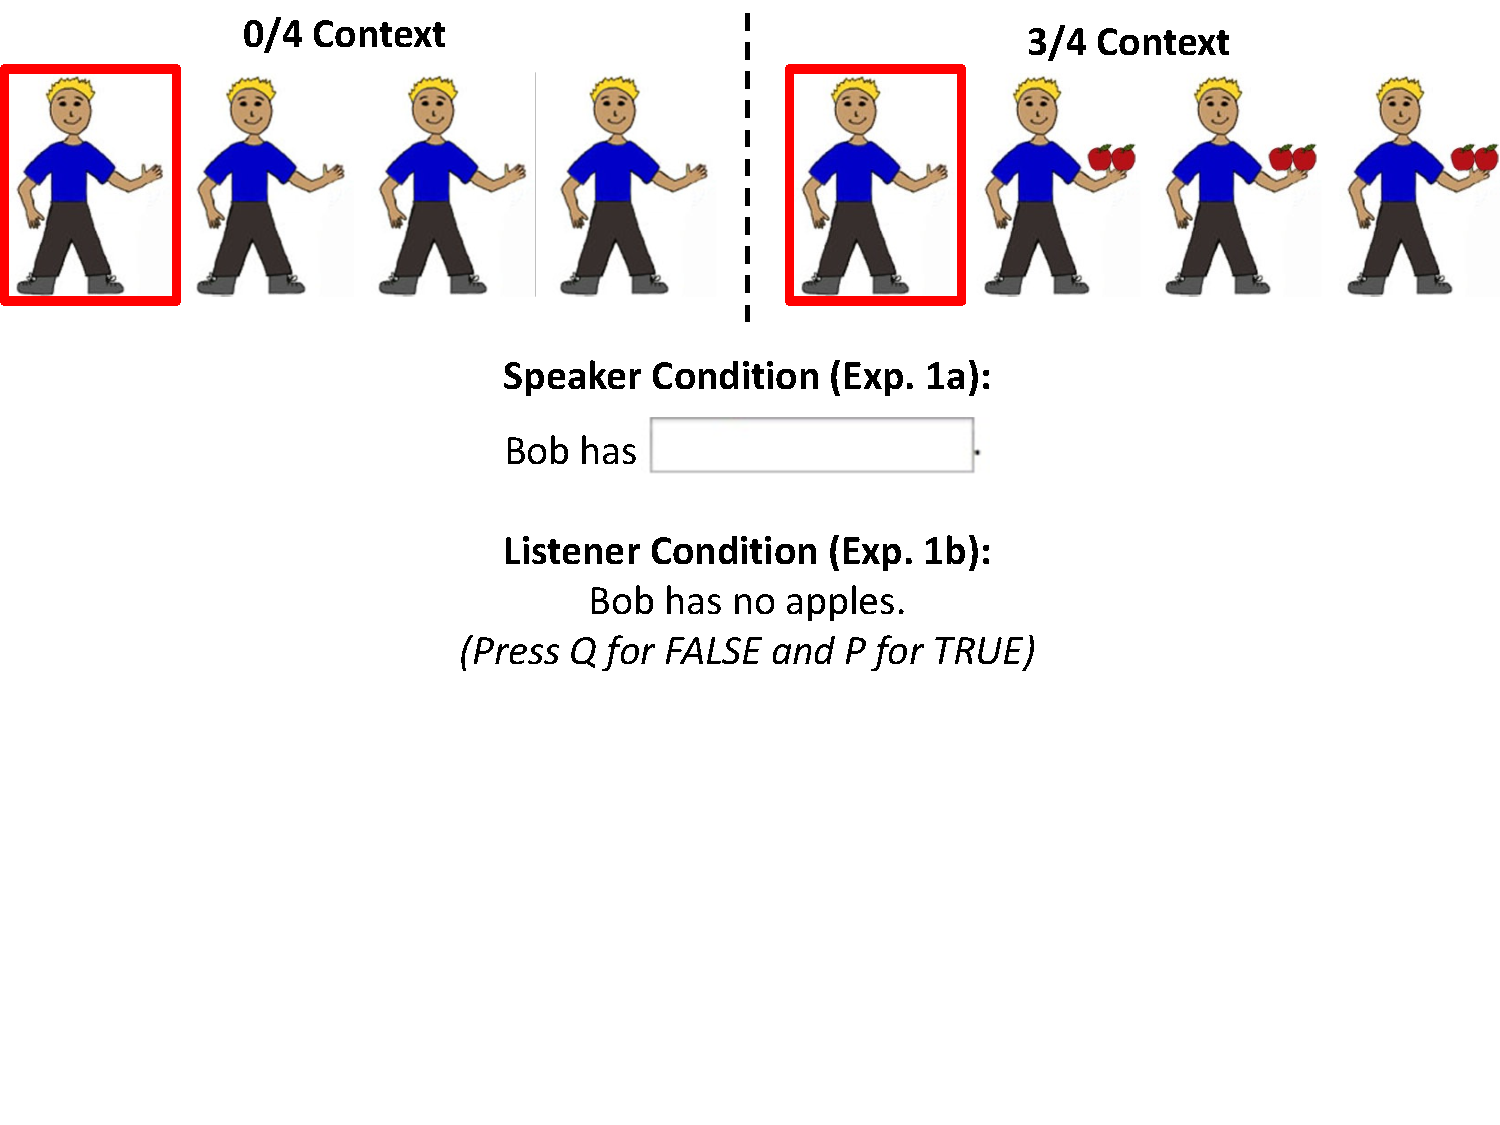
\includegraphics[width=6in]{figures/experiment1/trialfig_exp1.pdf}
\caption{\label{fig:exp1_trial} An example of a true negative trial with a 0/4 context (left) and a 3/4 context (right).  The sentence ``Bob has no apples'' in the 0/4 context is both uninformative (because the sentence is true of all of the characters) and irrelevant (because apples are not present in the context and therefore the QUD is unlikely to be about apples), whereas the same sentence in the 3/4 context is both informative and relevant. }
\vspace{-5mm}
\end{center} 
\end{figure}

Thirty-two trial items were created in which characters were shown holding either two of the same common, recognizable objects (``target items''; e.g., two apples), or holding nothing (see Figure \ref{fig:exp1_trial}). 

Each participant saw trials in which different proportions of characters were holding target items (context condition).  These contexts showed $\frac{0}{4}$, $\frac{1}{4}$, $\frac{2}{4}$, $\frac{3}{4}$, or $\frac{4}{4}$ of the characters holding objects. The order of characters was shuffled on each trial, with the referent of the sentence appearing in a random position. 

Participants saw each image paired with an incomplete sentence (e.g. ``[NAME] has $\rule{3cm}{0.15mm}$.''). In half of the trials, the highlighted character was holding target items (``item'' trials), and in half of the trials, the highlighted character was holding nothing (``nothing'' trials).  The experiment was fully crossed such that target characters appeared with or without target items an equal number of times in each context type. 

\subsubsection{Procedure}

Experiment 1a can be viewed at \url{http://anordmey.github.io/negatron/experiments/experiment1/speakers/negatron.html}. Presentation and randomization of stimuli and the collection of reaction time was controlled using javascript and jquery version 1.11.1. Experiment code can be found in the supplemental files at  \url{https://github.com/anordmey}.

 Participants were first presented with a brief overview screen explaining that they would play a language game.  Once participants accepted the task, they were randomly assigned to Experiment 1a (speakers) or Experiment 1b (listeners) and saw more detailed instructions which explained the task and informed them that they could stop at any time. 

Participants were told, ``First you will see four people. Pay attention to all four people until a red box appears around one of the people. When the red box appears, you will see an incomplete sentence below the pictures. The sentence that you see is about the picture with the box around it. Your job is to finish the sentence using only a few words. You should complete the sentence in a way that would help someone else identify the character in the red box if they saw the pictures in a different order.'' After these instructions, participants were shown an example trial which showed them an example of a positive trial, and explained again ``Remember, your job is to complete the sentence so that another person might be able to identify the character if they saw these pictures in a different order.''

Participants saw an array of four pictures on each trial: The target pictures and three context pictures presented in a random horizontal arrangement.  Participants looked at these pictures for four seconds, at which point a red box appeared around one of the pictures.  One second later, an incomplete sentence appeared, with a textbox for participants to complete the sentence. 

\subsubsection{Data Processing} 

Affirmative responses labeling the target feature were coded as ``positive'' (e.g., ``apples,'' ``two apples,'' ``red apples,'' etc.).  Responses negating the target feature (e.g., ``no apples'') were coded as ``negative.''  All other responses (e.g. descriptions of the characters' clothing or hair color, as well as other types of positive or negative utterances) were coded as ``other.''   Codes were hand-checked to ensure that label synonyms or spelling errors were coded correctly. The raw data for this experiment and all experiments reported in this manuscript can be found at \url{https://github.com/anordmey/negatron}, which includes the full responses of all participants in the speaker experiments. 

We calculated the proportion of positive sentences describing characters who possessed target items, and the proportion of negative sentences describing characters with nothing, creating probability distributions for true positive and true negative utterances in each context.  We then used this distribution to calculate the surprisal of hearing a true positive or true negative sentence for each context. Surprisal (or ``self-information'' $I$) for a sentence $s$ is defined as

\begin{equation}
\label{eq:surprise}
I(s) = -\log(P(s)).
\end{equation}

\subsection{Results \& Discussion}

\begin{figure}[t]
\begin{center} 
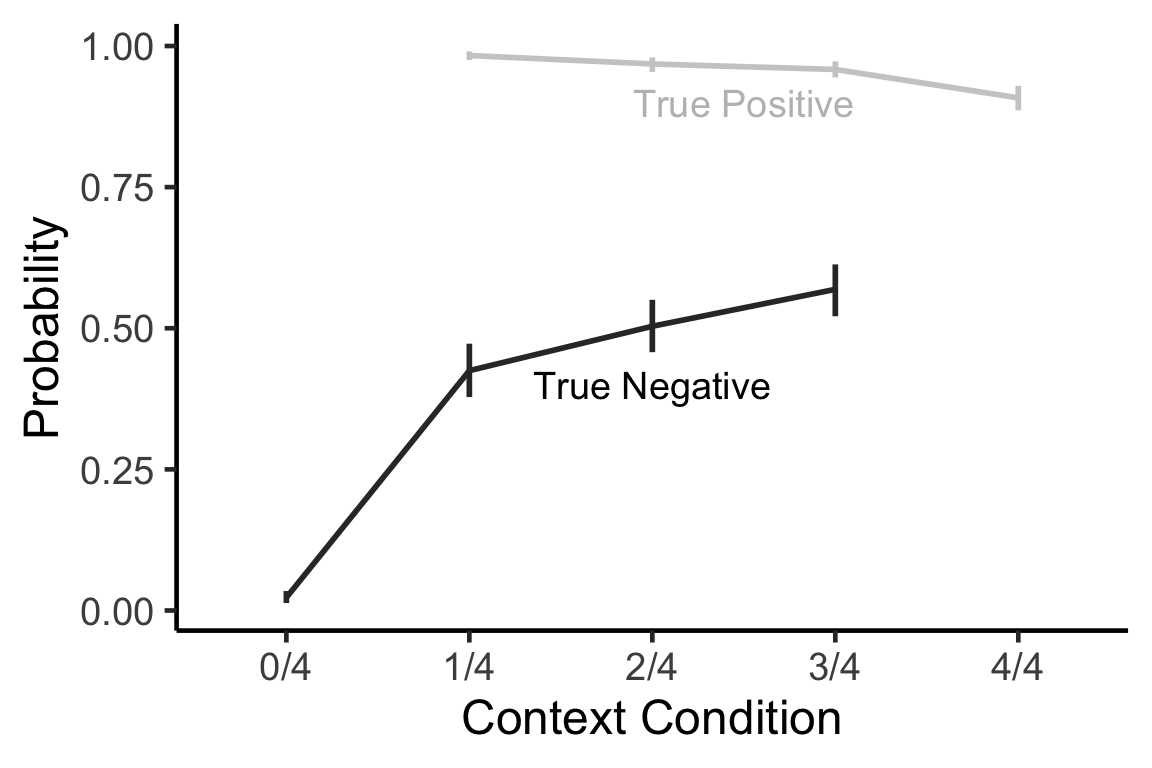
\includegraphics[width=4in]{figures/experiment1/speaker_probs.png}
\caption{\label{fig:exp1_speakerprobs} Probability of producing negative sentences on ``nothing'' trials (i.e., true negatives) and positive sentences on ``item'' trials (i.e., true positives) across different contexts. Negative sentences are shown in black, and positive sentences in grey.  The context is notated by a fraction representing the number of characters in the context who held target items. Error bars show 95\% confidence intervals computed by non-parametric bootstrapping.  }
\end{center} 
\end{figure}

\begin{figure}[t]
\begin{center} 
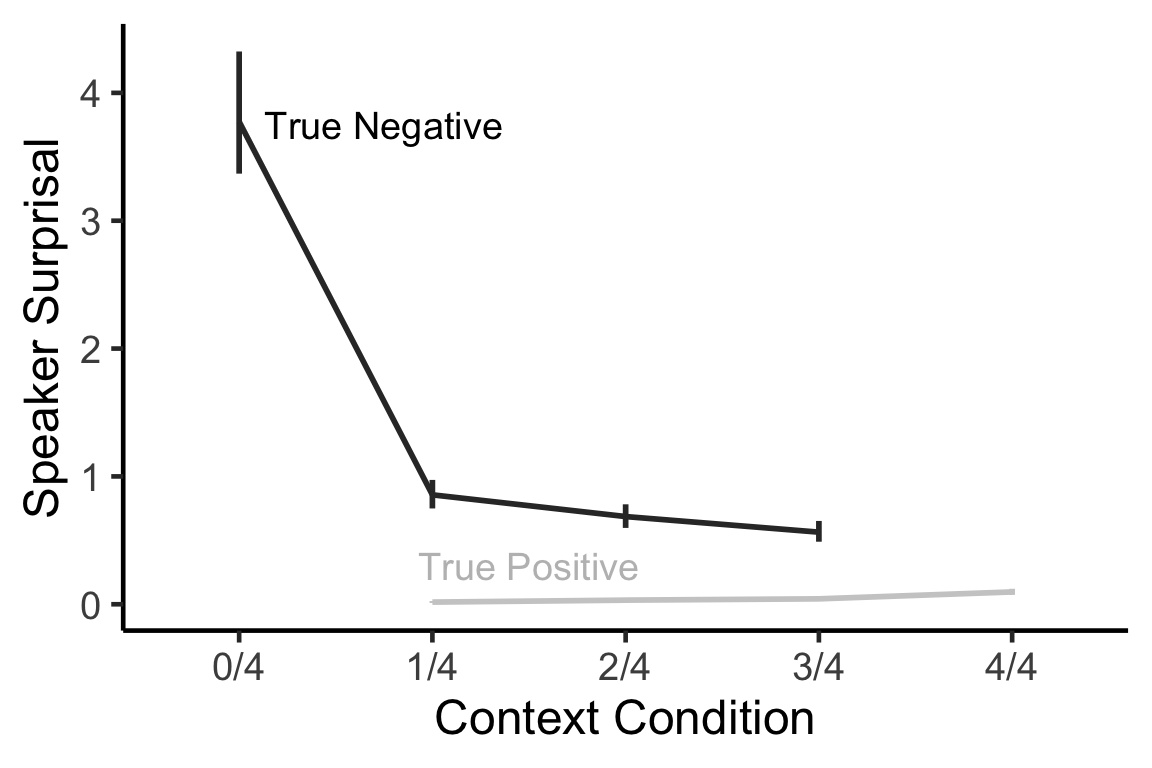
\includegraphics[width=4in]{figures/experiment1/speaker_surprisal.png}
\caption{\label{fig:exp1_speakersurprise} Surprisal for true positive and true negative sentences across different contexts. Negative sentences are shown in black, and positive sentences in grey.  The context is notated by a fraction representing the number of characters in the context who held target items. Error bars show 95\% confidence intervals computed by non-parametric bootstrapping.  }
\end{center} 
\end{figure}

Figure \ref{fig:exp1_speakerprobs} shows the proportion of participants who produced affirmative sentences to describe the presence of target items (true positives), and negation to describe the absence of target items (true negatives). A table of the precise probabilities displayed in this table can be found in the supplemental materials. Participants produced more true positive utterances about the presence of target items than true negative utterances about the absence of target items. As the number of characters in the context with target items increased, however, participants became slightly less likely to produce true positive utterances about referents with target items, and more likely to produce true negative utterances about characters without target items (see Figure \ref{fig:exp1_speakerprobs}). There is a large jump in the production of true negative utterances between the $\frac{0}{4}$ context, where only 2\% of responses were negations of the target item, and the $\frac{1}{4}$ context, where 42\% of responses were negative. 

To evaluate the reliability of these patterns, we fit two separate binomial mixed-effects models: 1) a model fit only to negative utterances describing the absence of a target item (i.e., true negatives), and 2) a model fit only to positive utterances describing the presence of positive items (i.e., true positives). To test the effect of informativeness, we coded context as a continuous variable, e.g. the proportion of characters in the context with target items. To test the effect of relevance, we created a dummy code to separately test for the effects of the  $\frac{0}{4}$ context compared to all of the other contexts (i.e., the contexts where discussing the presence or absence of apples is relevant).\footnote{All mixed-effects models used the maximal convergent random effects structure \cite{barr2013} and were fit using the lme4 package version 1.1-27 in R version 4.1.1. Significance for binomial mixed-effects models was derived in glmer() using the Wald Z test and for linear mixed models was calculated using the standard normal approximation to the t distribution \cite{barr2013}.}.

The first model explored the effect of context on the probability of producing a true negative utterance on ``nothing'' trials \footnote{The model specification was as follows: \texttt{negation $\sim$  relevant context + continuous context + (1~\textbar~subject) +  (1~\textbar~item)}.} We found a significant positive linear effect of context, with the probability of producing a negative sentence increasing as the proportion of characters with target items increases ($\beta= 2.30$, $p< .001$), indicating a significant effect of informativeness on the production of negative sentences. We also found that participants were significantly less likely to produce negative utterances in the $\frac{0}{4}$ compared to the other context conditions, indicating an effect of relevance ($\beta= -4.83$, $p< .001$). Comparing this model to an identical model without the relevance factor indicates that including relevance as a factor in the model significantly improves model fit ($\chi(1)= 487.63, p < .001$). 

The second model tested the effect of context on the probability of producing a true positive utterance on ``item'' trials.\footnote{The model specification was as follows: \texttt{positive $\sim$  continuous context + (1~\textbar~subject) +  (1~\textbar~item)}.} We found a significant \textit{negative} linear effect of context ($\beta= -2.87$, $p< .001$), indicating that the probability of producing a positive utterance decreases as the proportion of characters with target items increases. The findings of both models together suggest that the probability of producing both true positive and true negative utterances is influenced by the informativeness of that utterance in context.

These findings suggest that the production of both negative \textit{and} positive sentences was influenced by the surrounding context, although the effect on negative sentences was more pronounced. This supports our hypothesis that speakers will produce informative utterances (i.e. produce sentences that are maximally effective at identifying the referent), because true positive utterances about the presence of target items are most informative when none of the other characters have target items (e.g. the $\frac{1}{4}$ context), whereas true negative utterances about the absence of target items are most informative when the other characters \textit{do} have target items (e.g. the $\frac{3}{4}$ context). We can also see the impact of informativeness in Figure \ref{fig:exp1_speakersurprise}, which shows the surprisal of true positive and true negative sentences, with surprisal decreasing for true negative sentences and increasing for true positive utterances as the number of characters with target items increases. 

The difference between the production of negation in the $\frac{0}{4}$ compared to the  $\frac{1}{4}$ demonstrates the impact of ``relevance''. This pattern is also seen clearly in the surprisal of utterances produced, in Figure \ref{fig:exp1_speakersurprise}. The steep gap in surprisal between the  $\frac{0}{4}$ and the  $\frac{1}{4}$ contexts is driven by the fact that almost no participants produced negation in the  $\frac{0}{4}$ context. In this context, because there are no e.g. ``apples'' in the context, the QUD is unlikely to pertain to apples, and therefore apples are unlikely to be mentioned by the speaker. In contrast, the $\frac{1}{4}$ context is more likely to give rise to a polar QUD where mentioning the presence or absence of e.g. ``apples'' is a relevant response. 

\subsubsection{Post hoc Analyses}

In our analyses we coded utterances such as ``Bob has zero apples'' and ``Bob has nothing'' as ``other'' rather than ``negative" because we wanted to examine speaker utterances that were as close as possible to the utterances in the listener condition (Experiment 1b). Furthermore, our discussion of relevance makes specific predictions about the negation of the target item (e.g., a polar QUD licenses [\textit{has apples, has no apples}]) and it is less clear what QUDs license the response \textit{has nothing}. In an exploratory analysis, however, we found that including other instances of negation in our analysis (e.g., ``not apples'', ``without apples'', ``zero apples'', and ``has nothing'') does not change the pattern of results described above for negative sentences (i.e., significant effects of relevance, $\beta= -2.73$, $p< .001$, and informativeness, $\beta= 2.12$, $p< .001$). 

\section{Experiment 1b: Listeners, identical characters}

In Experiment 1b, participants viewed trials that were identical to the trials in Experiment 1b (Figure \ref{fig:exp1_trial})) except that instead of being asked to complete sentences, participants were shown a sentence of the form ``[NAME] [has/has no] [TARGET ITEM]'' and were asked to complete a sentence verification task, answering as quickly and accurately as possible whether the sentence was true of the identified referent. 

\subsection{Method}

\subsubsection{Participants} 

Participants were recruited for Experiment 1b at the same time as Experiment 1a. We restricted participation to individuals in the US and paid 50 cents for this 10 minute study. As described in Experiment 1a, after excluding participants who reported being under age 18 or having a native language other than English, n = 188 remained for analysis in Experiment 1b; of these, 92 were male and 95 were female, 1 declined to report gender, and ages ranged from 18-66+.

\subsubsection{Stimuli}

Participants saw sets of four characters identical to the images shown in Exp. 1a, except that instead of filling in a sentence to describe a character, participants completed a sentence verification task (see Figure \ref{fig:exp1_trial})). On each trial a sentence of the form ``[NAME] [has/has no] [TARGET ITEM]'' appeared.  Half of the sentences were positive and half were negative (sentence type), and they were paired with pictures such that half were true and half were false (truth value), resulting in four possible trial types (true positive, true negative, false positive, and false negative).  Because true positive and false negative sentences cannot occur in a $\frac{0}{4}$ context (i.e. the referent must have the target item in these trials), and true negative and false positive sentences cannot occur in a $\frac{4}{4}$ context, each trial type occurred in four possible contexts.  The experiment was fully crossed, with participants receiving eight true positive, eight false positive, eight true negative and eight false negative sentences distributed equally across context types in a randomized order over the course of the study.  

\subsubsection{Procedure}

Experiment 1b can be viewed at \url{http://anordmey.github.io/negatron/experiments/experiment1/listeners/negatron.html}. Presentation and randomization of stimuli and the collection of reaction time was controlled using javascript and jquery version 1.11.1. Experiment code can be found in the supplemental files at  \url{https://github.com/anordmey}.

On each trial, participants saw an array of four pictures for four seconds, at which point a red box appeared around one of the pictures. One second later, a sentence about that picture appeared. Participants were told to read the sentence and respond as quickly and accurately as possible with a judgment of whether it was true or false when applied to the highlighted picture (by pressing either `P' or `Q').  We used javascript to record reaction times for each trial, measured as the time from when the sentence was presented to the moment when the response was made.

Participants first saw eight positive sentence practice trials with feedback about incorrect responses before beginning the test trials. The practice trials showed four people holding objects in various colors, and the target sentence described the color of the referent item in a way that was accurate or inaccurate. On the test trials, participants saw the same arrays of pictures shown in Experiment 1a. 

\subsubsection{Data Processing} 

We excluded two participants for having an overall accuracy below 80\%, which left a total of n = 186 participants for analysis. At the trial level, we excluded trials with RTs greater than 3 standard deviations from the log-transformed mean, a criterion established in our previous experiments \cite{nordmeyer2014}. 

\subsection{Results \& Discussion}

\begin{figure}[t]
\begin{center} 
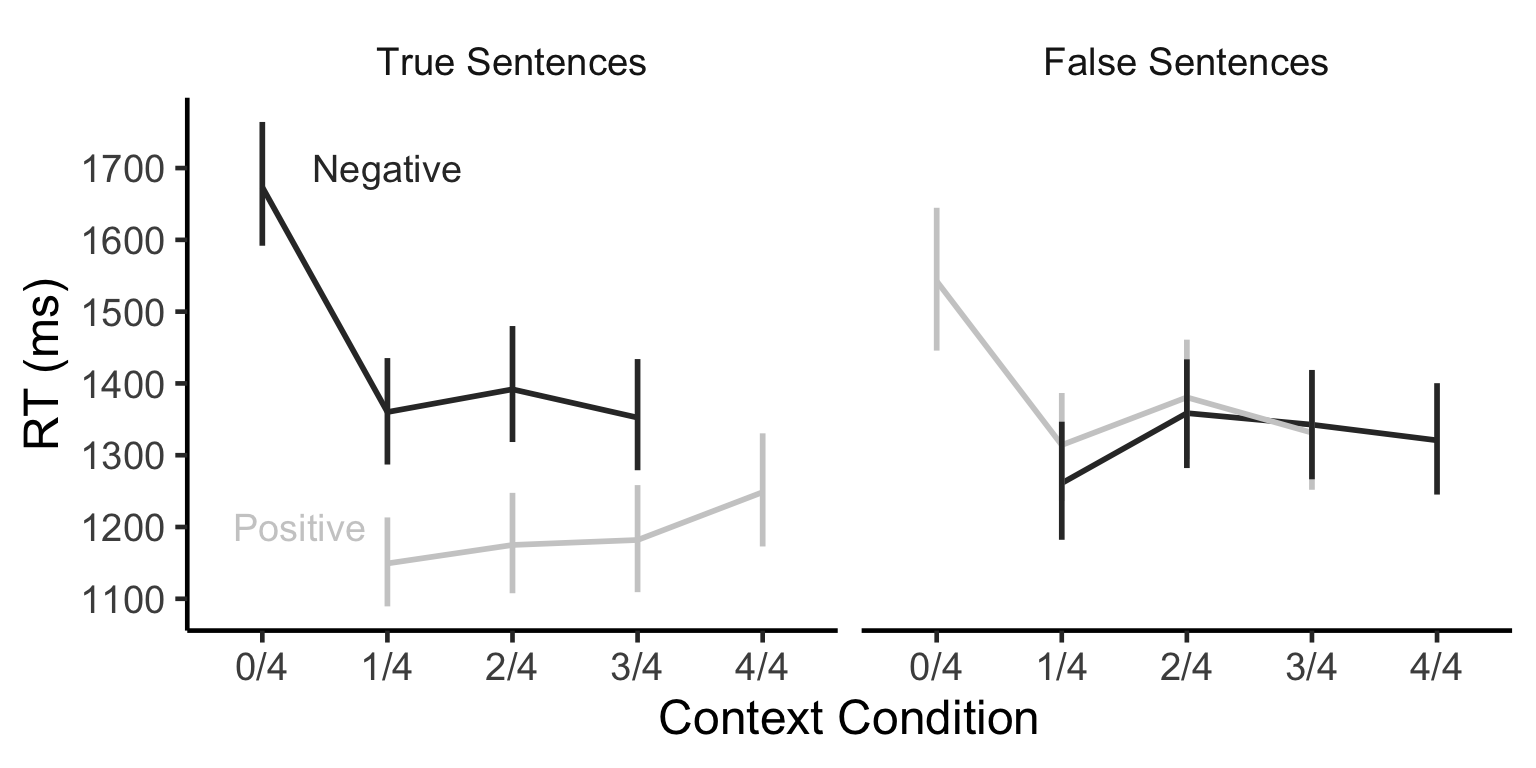
\includegraphics[width=6in]{figures/experiment1/listener_rts.png}
\caption{\label{fig:exp1_listenerrt} Reaction times for each trial type across different conditions. Responses to true sentences are shown on the left, and false sentences are shown on the right.  Negative sentences are shown in black, and positive sentences in grey.  The context is notated by a fraction representing the number of characters in the context who held target items. Error bars show 95\% confidence intervals computed by non-parametric bootstrap.}
\end{center} 
\end{figure}

Overall accuracy on this task was very high, with participants responding correctly on 98\% of true positive trials, 92\% of true negative trials, 95\% of false positive trials, and 96\% of false negative trials.  Participants' reaction times can be seen in Figure \ref{fig:exp1_listenerrt}. Participants were fastest to respond to true positive sentences, and slowest to respond to true negative sentences in all context conditions. Replicating previous findings \cite{hclark1972}, we also see an interaction between polarity and truth value, such that participants are slowest to respond to true negatives and false positives. Focusing on responses to true sentences (which can be directly compared to the speaker responses in Experiment 1b, where participants were asked to produce true sentences), listeners' reaction times to true negative sentences mirrored the surprisal of true negative sentences in Experiment 1a, with participants responding slowest to true negatives in the $\frac{0}{4}$ context.

We fit a linear mixed-effects model to examine the interaction between sentence type (positive or negative), truth value (true or false), and context as predictors of reaction time.\footnote{The model specification was as follows: \texttt{RT $\sim$ sentence~$\times$~truth~$\times$~context + (sentence~\textbar~subject) +  (sentence~\textbar~item)}.} All model coefficients are shown in Table \ref{tab: exp1_listenermodel}. In addition to main effects of sentence type ($\beta= -205$, $p< .001$) and truth value ($\beta= -372$, $p< .001$), there was an interaction between sentence type and truth value such that true positive sentences elicited the fastest responses and true negative sentences elicited the slowest responses ($\beta= 692$, $p< .001$). The model showed a significant negative linear effect of context, with reaction times decreasing as the proportion of characters with target items increased ($\beta= -238$, $p< .001$) and a significant three-way interaction between sentence type, truth value, and context ($\beta= -839$, $p< .001$).  This three-way interaction reflects the fact that both true negatives and false positives in the $\frac{0}{4}$ are strikingly slower than any other sentence type in any context. Both true negative and false positive sentences in the $\frac{0}{4}$ context are using the word e.g. ``apples'' to describe a scene in which there are no apples present. Although our focus here is on responses to true sentences, the slow reaction times for both true negative and false positive sentences suggests that listeners expect speakers to describe relevant features of the context even when the sentence is false. 

To explore the separate effects of relevance (i.e., the effect of the $\frac{0}{4}$ context compared to the others) and informativeness (i.e. the linear effect of context) on responses to true utterances, we fit two separate models to reaction times in response to true positive and true negative utterances.\footnote{Model specification for true negative model: \texttt{rt $\sim$  relevance context + numeric context + (relevant context + numeric context~\textbar~subject) +  (relevant context + numeric context~\textbar~item)}; model specification for true positive model: \texttt{rt $\sim$  numeric context + (numeric context~\textbar~subject) +  (numeric context~\textbar~item)}.} We found a significant effect of relevance on reaction times for negative utterances, with the $\frac{0}{4}$ context producing significantly slower reaction times compared to the relevant contexts ($\beta= 331$, $p< .001$). We did not find a significant linear effect of context above and beyond the effect of the  $\frac{0}{4}$ context ($\beta= -4.01$, $p = .96$). We did, however, find a significant positive linear effect of context on the the reaction time to respond to positive sentences ($\beta= 123$, $p = .02$), indicating a significant effect of informativeness on RTs to positive sentences, but not negative sentences. 

\begin{table}
\caption{\label{tab: exp1_listenermodel} Model output from a mixed-effects model predicting listeners' reaction times in response to sentences in different contexts.}
\begin{center}
% \small\addtolength{\tabcolsep}{-5pt}
\begin{tabular}{rrrr}
  \hline
 & Coefficient & Std. err. & $t$ \\ 
  \hline
Intercept & 1483 & 42 & 35.27 \\ 
  Sentence (Negative) & -205 & 37 & -5.51  \\ 
  Truth (True) & -372 & 37 & -10.00 \\
  Context & -238 & 43 & -5.50 \\ 
  Sentence $\times$ Truth & 692 & 53 & 12.99 \\
  Sentence $\times$ Context & 310 & 61 & 5.09 \\
  Truth $\times$ Context & 366 & 61 & 6.04 \\
  Sentence $\times$ Truth $\times$ Context & -839 & 87 & -9.68 \\
   \hline
\end{tabular}
\end{center}
\end{table}

\subsubsection{Comparing Speakers and Listeners across Experiment 1}

\begin{figure}[t]
\begin{center} 
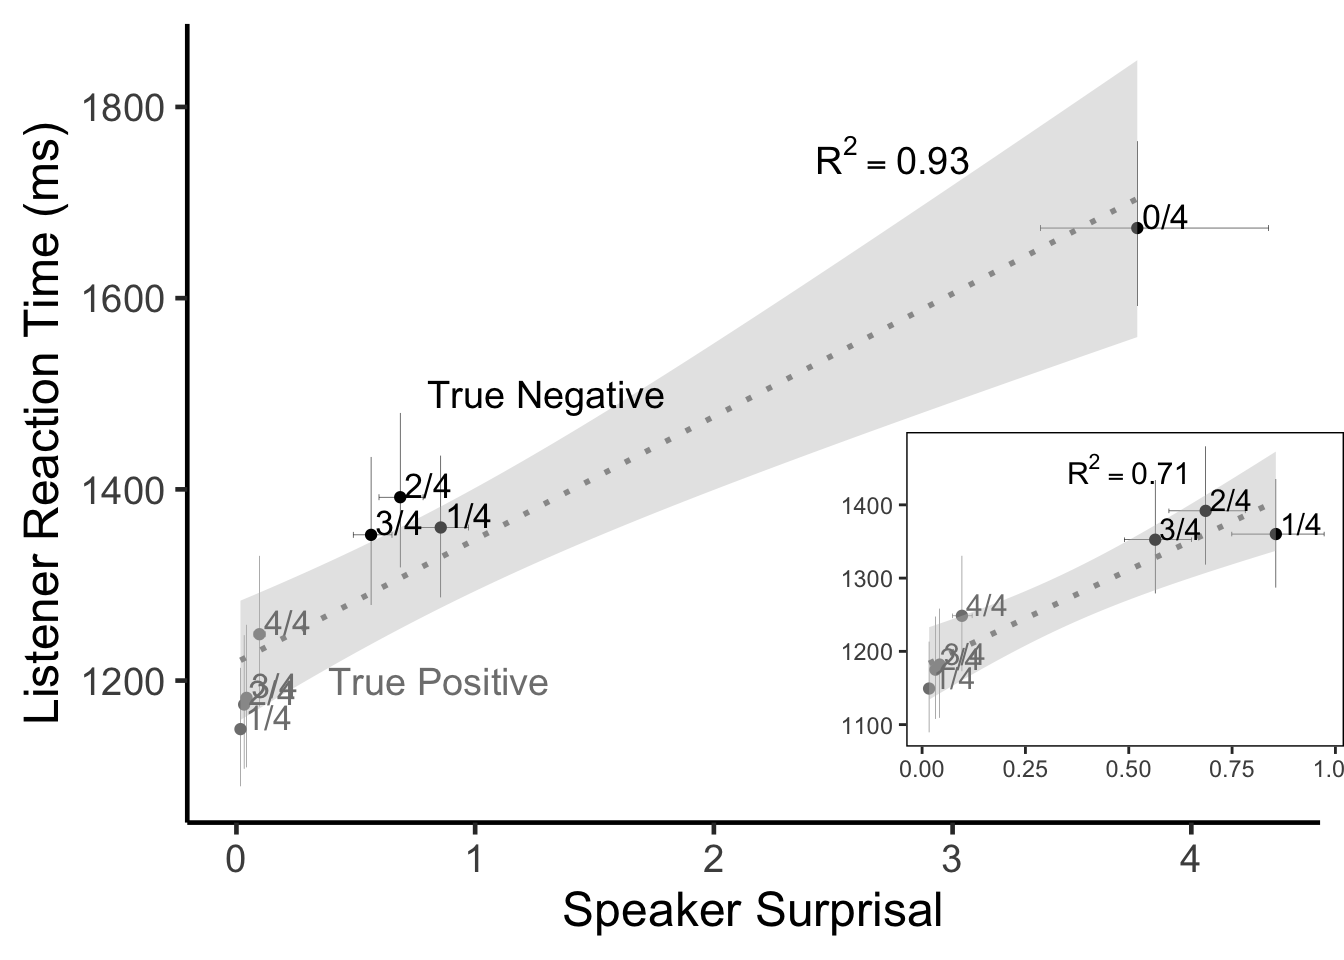
\includegraphics[width=6in]{figures/experiment1/speaker_v_listener.png}
\caption{\label{fig:exp1_scatter} Reaction times in the listener condition plotted by surprisal in the speaker condition. Each point represents a measurement for sentence type and context. Negative sentences are shown in black, and positive sentences in grey. Error bars on the horizontal and vertical axes represent 95\% confidence intervals on their respective measures. The gray band shows the linear regression and  95\% confidence region for all conditions. The inset graph zooms in on the linear regression and 95\% confidence region for data excluding the outlying 0/4 condition.}
\end{center} 
\end{figure}

To test our hypothesis that processing times are a function of listeners' expectations about what a speaker will say, we regressed the mean reaction time in response to true positive and negative utterances in each condition against the surprisal for the same utterances (Figure \ref{fig:exp1_scatter}).  There was a significant positive relationship between surprisal and reaction time for true negative sentences, $R^2=.89$, $p<.001$, supporting our prediction that the effects of context on reaction time reflect differences in how speakers would describe the same stimuli. This relationship between surprisal and reaction time for true negative sentences holds even with the outlying $\frac{0}{4}$ context removed from analysis ($R^2=.89$, $p = .002$).


\section{Experiment 2a: Speakers, varied characters}

In Experiment 1 we demonstrated that the probability of speakers (participants in Exp. 1a) producing negations was influenced by both the relevance (i.e. whether the context promotes a polar QUD) as well as the informativeness (i.e. how well a negation identified the referent in context) of these utterances in context. In addition, we demonstrated that the processing time for listeners (participants in Exp. 1b) to respond to negative sentences was highly correlated to the surprisal of speakers' productions of these utterances. 

In Experiment 1 we increased the probability of negation by \textit{only} varying the presence and absence of target items across characters. Would participants continue to use negation in a more natural context where other features existed to disambiguate the characters, and would the presence of these alternative features influence the effect of relevance and informativeness? In Experiment 2 we explored this question by varying both the shirt and hair color of the characters within each trial, in addition to varying the presence and absence of target items between trials. Experiment 2a was identical to Experiment 1a, except the trials in Exp. 2a were altered to add these additional features to characters. 

\subsection{Method}

\subsubsection{Participants} 

Participants were recruited for Experiment 2a and 2b in tandem, and were randomly assigned to one of the two experiments at the start of data collection. We recruited a planned sample of 500 participants to participate in these online experiments through the Amazon Mechanical Turk (mTurk) website. We restricted participation to individuals in the US and paid 50 cents for this 10 minute study. 5 participants were rejected for indicating that they were under 18 after completing the experiment, and an additional 16 participants were excluded for indicating that their native language was not English. Of the remaining 479 participants (across Exp 2a and Exp 2b), n = 233 completed Exp. 2a (speakers); of these, 111 were male and 122 were female, and ages ranged from 18-66+. 

\subsubsection{Stimuli}

\begin{figure}[t]
\begin{center} 
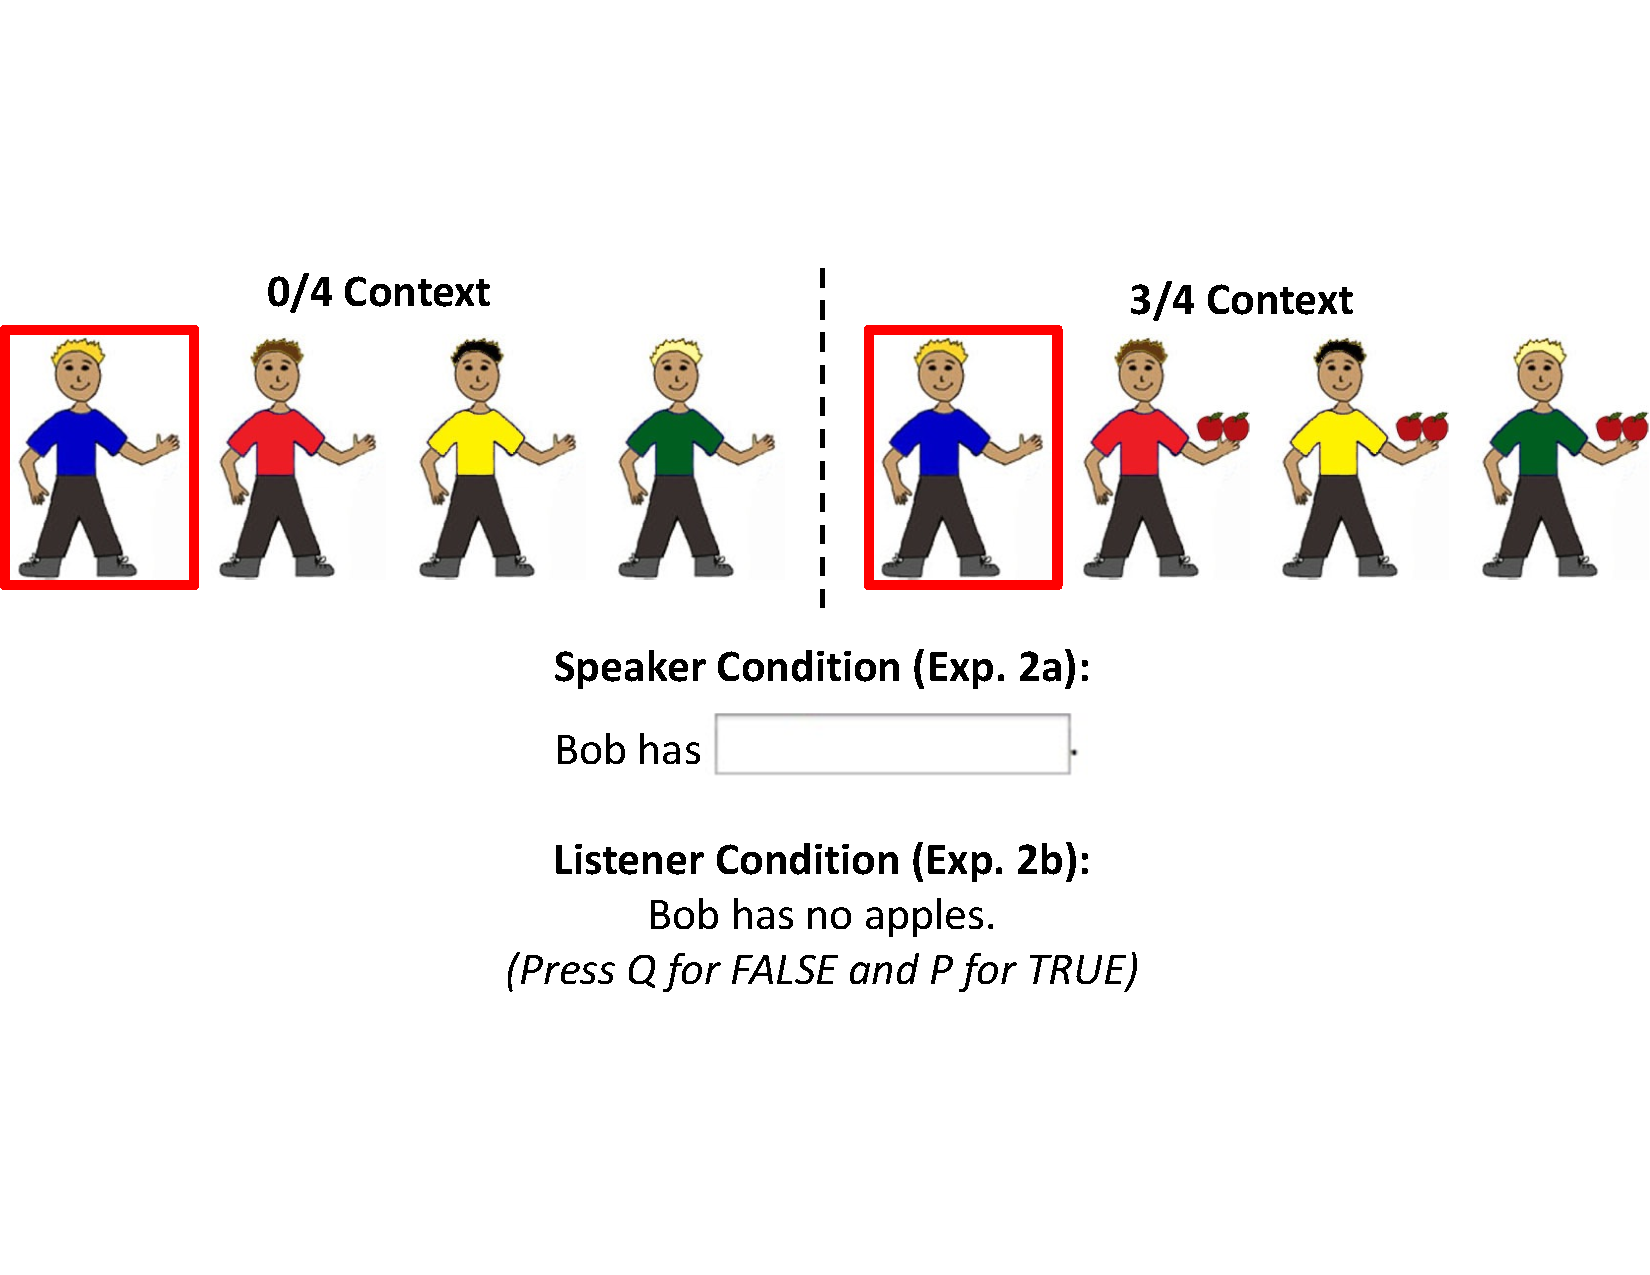
\includegraphics[width=6in]{figures/experiment2/trialfig_exp2.pdf}
\caption{\label{fig:exp2_trial} An example of a true negative trial with a 0/4 context (left) and a 3/4 context (right).  The sentence ``Bob has no apples'' in the 0/4 context is both uninformative (because the sentence is true of all of the characters) and irrelevant (because apples are not present in the context and therefore the QUD is unlikely to be about apples), whereas the same sentence in the 3/4 context is both informative and relevant. }
\vspace{-5mm}
\end{center} 
\end{figure}

Stimuli were identical to the stimuli in Exp. 1a except that within each trial characters' shirt and hair colors also varied, providing other referential possibilities for speakers (see Figure \ref{fig:exp2_trial})). 

\subsubsection{Procedure}

Experiment 2a can be viewed at \url{http://anordmey.github.io/negatron/experiments/experiment2/speakers/negatron.html}. Presentation and randomization of stimuli and the collection of reaction time was controlled using javascript and jquery version 1.11.1. Experiment code can be found in the supplemental files at  \url{https://github.com/anordmey}.

Although the task was identical to the ``complete the sentence'' task in Experiment 1a, we altered the instructions slightly to emphasize that participants should not refer to the position of the character in the array, instead of emphasizing the ability for a listener to identify the referent. Participants were told, ``First you will see four people. Pay attention to all four people until a red box appears around one of the people. When the red box appears, you will see an incomplete sentence below the pictures.The sentence that you see is about the picture with the box around it. Your job is to finish the sentence using only a few words. Please avoid using descriptions of the person's position relative to other characters.'' After these instructions, participants were shown the same example trial as in Experiment 1a, and told again ``Please avoid using descriptions of the person's position relative to other characters. So, for example, do not complete the sentence by saying "second to the right".

\subsubsection{Data Processing} 

We followed the same coding procedure in Exp. 2a as we did in Exp. 1a. As in Exp. 1a, we calculated the proportion of positive sentences describing characters who possessed target items, and the proportion of negative sentences describing characters with nothing, creating probability distributions for true positive and true negative utterances in each context and using these distributions to calculate the surprisal of hearing a true positive or true negative sentence for each context. 


\subsection{Results \& Discussion}

\begin{figure}[t]
\begin{center} 
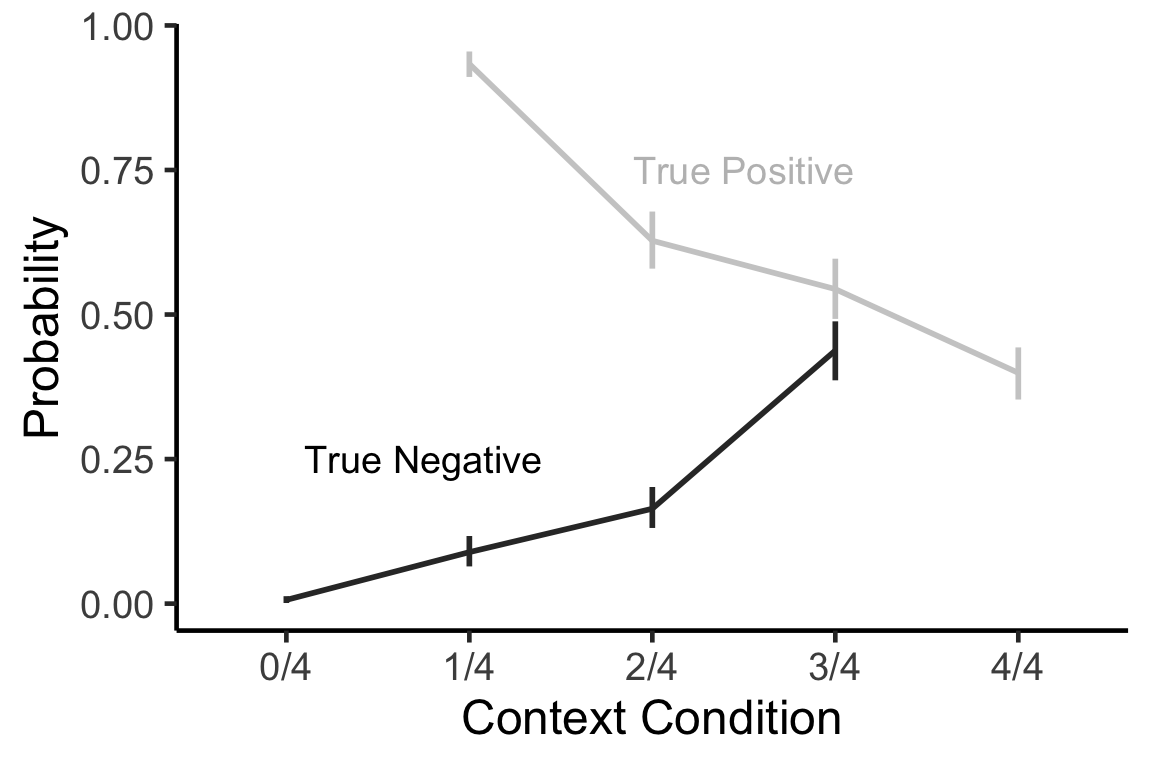
\includegraphics[width=4in]{figures/experiment2/speaker_probs.png}
\caption{\label{fig:exp2_speakerprobs} Probability of producing negative sentences on ``nothing'' trials (i.e., true negatives) and positive sentences on ``item'' trials (i.e., true positives) across different contexts. Negative sentences are shown in black, and positive sentences in grey.  The context is notated by a fraction representing the number of characters in the context who held target items. Error bars show 95\% confidence intervals computed by non-parametric bootstrapping.  }
\end{center} 
\end{figure}

\begin{figure}[t]
\begin{center} 
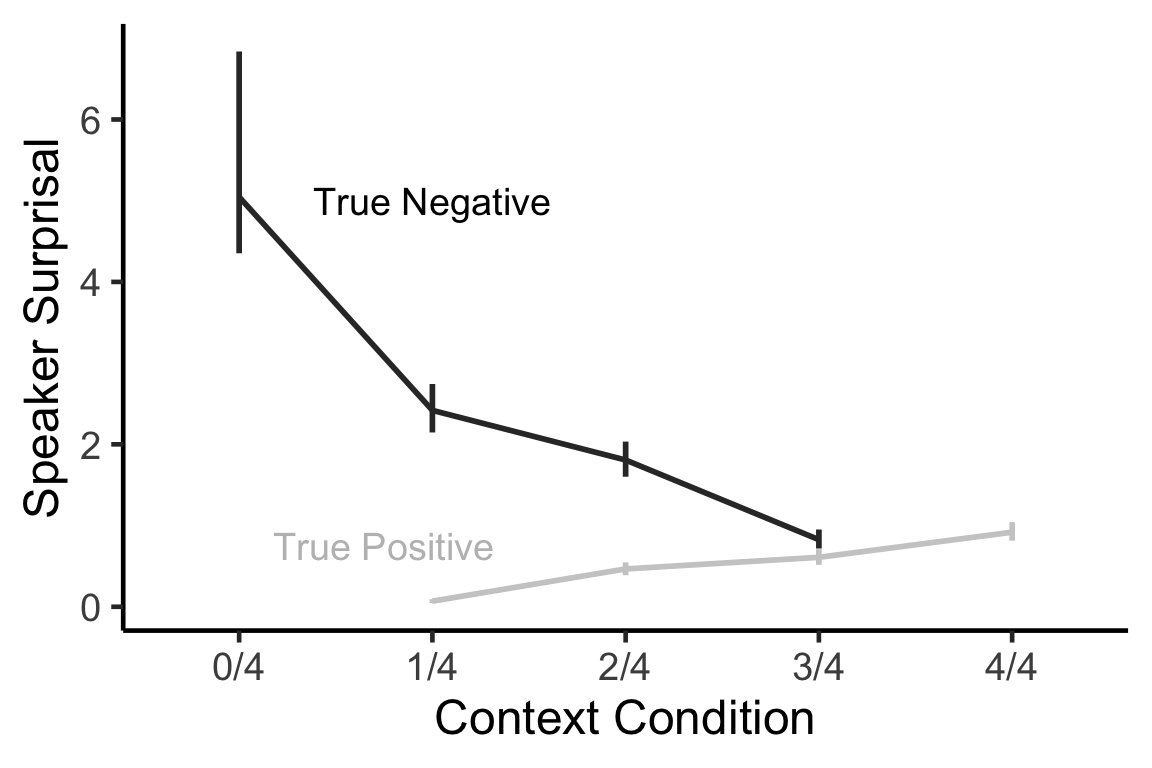
\includegraphics[width=4in]{figures/experiment2/speaker_surprisal.png}
\caption{\label{fig:exp2_speakersurprise} Surprisal for true positive and true negative sentences across different contexts. Negative sentences are shown in black, and positive sentences in grey.  The context is notated by a fraction representing the number of characters in the context who held target items. Error bars show 95\% confidence intervals computed by non-parametric bootstrapping.  }
\end{center} 
\end{figure}


Figure \ref{fig:exp2_speakerprobs} shows the proportion of participants who produced affirmative sentences to describe the presence of target items (true positives), and negation to describe the absence of target items (true negatives). A table of the precise probabilities displayed in this table can be found in the supplemental materials. As in Experiment 1a, the probability of producing true negative utterances decreases and the probability of of producing true positive utterances increases as the number of characters with target items increases.

As in Exp. 1a, we fit two separate binomial mixed-effects models: 1) a model fit only to negative utterances, and 2) a model fit only to positive utterances. To test the effect of informativeness, we coded context as continuous, e.g. the proportion of characters in the context with target items. To test the effect of relevance, we created a dummy code to separately test for the effects of the  $\frac{0}{4}$ context compared to all of the other contexts (i.e., the contexts where discussing the presence or absence of apples is relevant). 

For the first model described above, we tested the effect of context on the probability of producing a true negative utterance on ``nothing'' trials.\footnote{The model specification was as follows: \texttt{negation $\sim$  relevant context + continuous context + (1~\textbar~subject) +  (1~\textbar~item)}.} We  found a significant effect of the relevant contexts, indicating that participants were less likely to produce negative sentences in the $\frac{0}{4}$ context compared to the other contexts ($\beta= -1.19$, $p = .015$). This finding suggests that relevance has a significant effect on the production of true negative sentences. We also found a significant positive linear effect of context, with the probability of producing a negative sentence increasing as the proportion of characters with target items increases ($\beta= 7.30$, $p< .001$), indicating a significant effect of informativeness on the production of negative sentences. Comparing this model to an identical model without the relevance factor indicates that including relevance as a factor in the model significantly improves model fit ($\chi(1)= 7.23, p = .007$). 

The second model tested the effect of context on the probability of producing a true positive utterance on ``item'' trials.\footnote{The model specification was as follows: \texttt{positive $\sim$  continuous context + (1~\textbar~subject) +  (1~\textbar~item)}.} We found a significant \textit{negative} linear effect of context ($\beta= -5.5$, $p< .001$), indicating that the probability of producing a positive utterance decreases as the proportion of characters with target items increases. The findings of both models together suggest that the probability of producing both true positive and true negative utterances is influenced by the informativeness of that utterance in context.

A key difference between Experiment 1a and Experiment 2a is the \textit{relative} informativeness of describing the presence or absence of the target item, as opposed to describing e.g. shirt or hair color. In Experiment 1a, where all of the characters were identical, descriptions of clothing color were always relatively uninformative (because they were true of all characters in a given trial). That is, in Experiment 1a, negative utterances on ``nothing'' trials were therefore at least as informative as describing shirt color in the $\frac{1}{4}$, $\frac{2}{4}$, and $\frac{3}{4}$ contexts. Contrast this with Experiment 2a, where describing the color of a characters shirt is \textit{always} an informative utterance: the informativeness of a true negative utterance is only comparable to these competing utterances in the $\frac{3}{4}$ context. The effect of the informativeness of these competing utterances in the current study is reflected in the raw probabilities for the speaker data (Figure \ref{fig:exp2_speakerprobs}), where there is a jump in the probability of a true negative utterance between the $\frac{2}{4}$ and the $\frac{3}{4}$ context. In Experiment 1a, this sharp increase occurred between the $\frac{0}{4}$ and $\frac{1}{4}$ contexts -- again, the point where producing a true positive utterance becomes as informative as producing an utterance about e.g., shirt color. Overall, negation was produced less frequently in Experiment 2a (17\% true negative utterances across all context conditions) compared to Experiment 1a (38\% true negative utterances across all contexts), likely due in part to difference in the relative informativeness of negative utterances in Experiment 2. 

As in Experiment 1a, and consistent with our hypothesis that speakers will produce negative sentences that are relevant (i.e. producing an utterance that is a possible response to a likely QUD), negative sentences were almost never produced on “nothing” trials in the $\frac{0}{4}$ context. That is, “no apples” was a very rare production on trials where there weren’t any apples in the context; participants in this condition tended to produce affirmative sentences describing other features of the referent, such as their clothing or hair color. Participants only consistently produced negative utterances in the $\frac{1}{4}$ context, where at least one other character has target items, thus making Does boy X have apples? a likely QUD. Although the pattern of negation production looks different between Experiment 1 and Experiment 2 (as described in the paragraph above), when we look at speaker \textit{surprisal}, the two experiments show the same pattern. In both Experiment 1a and Experiment 2a, the \textit{surprisal} of producing a negative utterance is significantly higher in the $\frac{0}{4}$ than in any other context because the probability of producing a negative utterance in this context (i.e., mentioning the absence of an item that is seen nowhere in the context) is close to zero in both experiments. 

\subsubsection{Follow-up Analyses}

In Experiment 2a, we used the same coding scheme as in Experiment 1a, coding utterances such as “Bob has nothing” as “other” rather than “negative". Once again we examined how these coding decisions influenced our results in Experiment 2a. Consistent with our predictions, if we include other negations of the target item in our analysis (e.g., “not apples”, “without apples”, “zero apples”, etc.), the results of the speaker condition are the same as those reported above (i.e., significant effects of relevance and informativeness). If we also include instances of “nothing”, however, the effect of informativeness remains highly significant ($\beta = 6.55, p < .001$), but the effect of relevance is no longer significant ($\beta = 0.21, p = 0.50$). That is, “has no apples” is not a very relevant utterance in a context where no one else has apples, but “has nothing” is, perhaps, a relevant thing to say in the context of an experiment where people sometimes have objects and sometimes do not.

\begin{figure}[t]
\begin{center} 
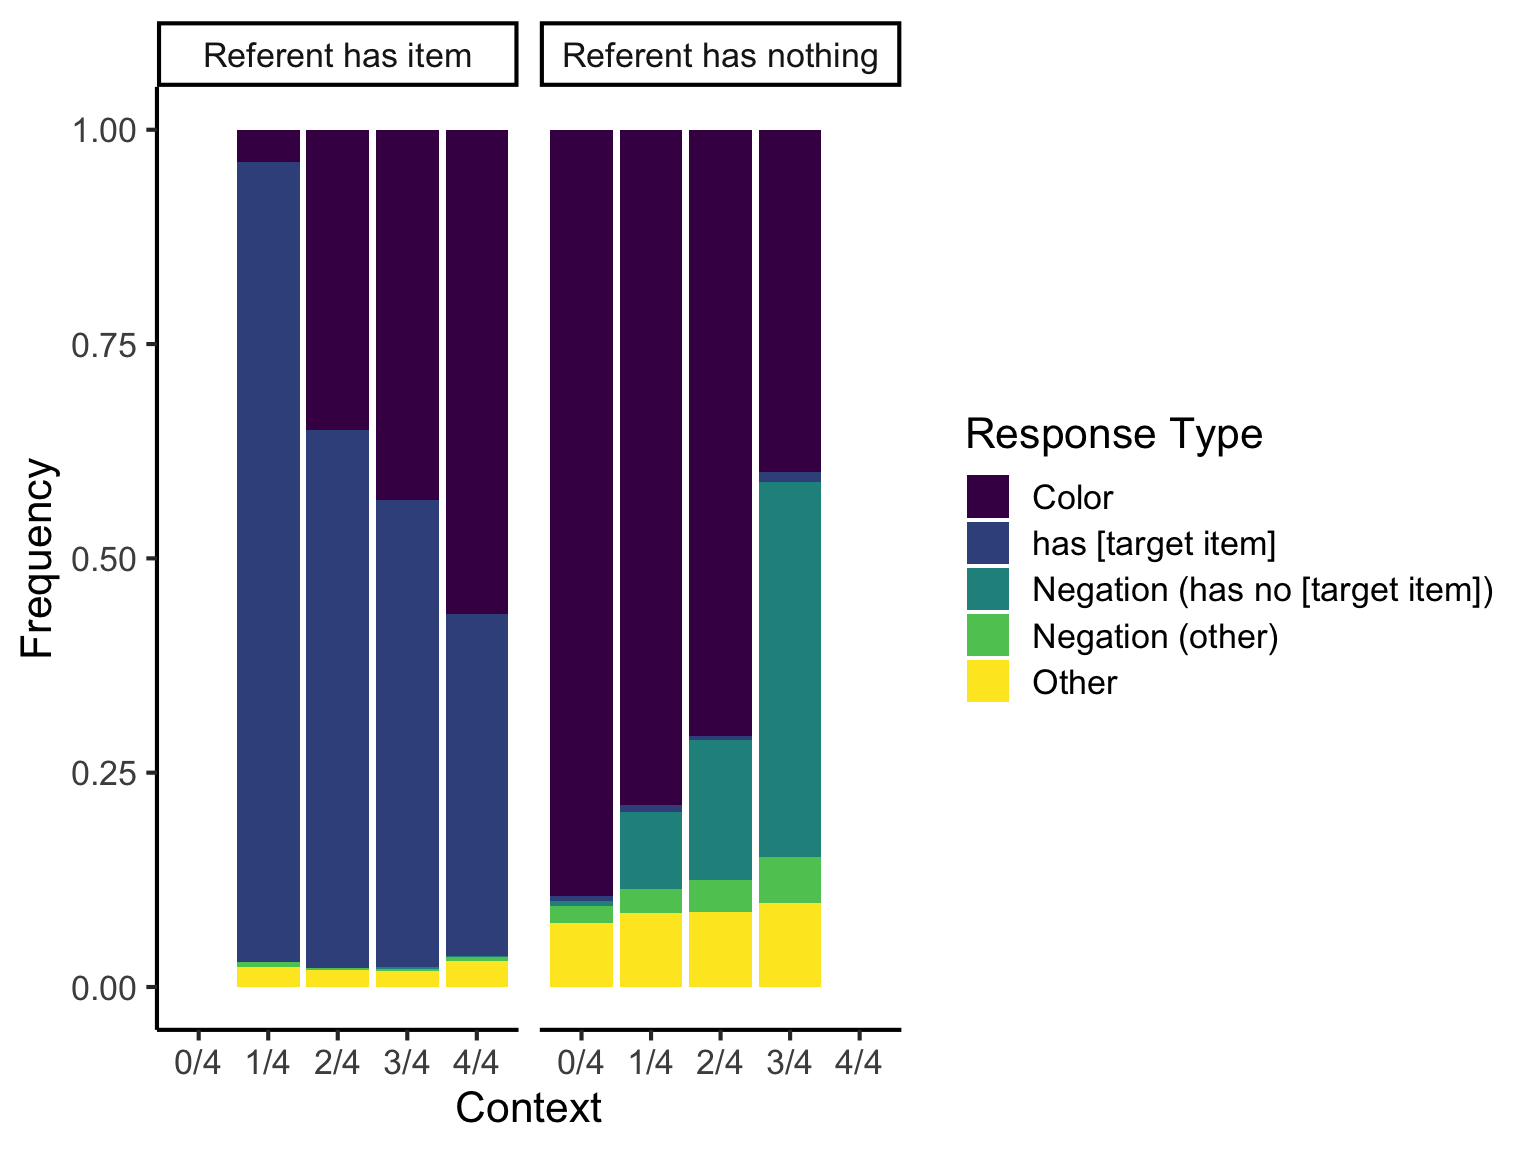
\includegraphics[width=6in]{figures/experiment2/speaker_responses_v1.png}
\caption{\label{fig:exp2_props} Categories of different types of speaker responses across the different context conditions. Purple bars (``Color'' responses) represent the proportion of participants who relied on descriptions of color (i.e. hair or shirt color) to describe the referent. Dark blue bars (the ``has [target item]'' responses) on the ``referent has item'' trials represent affirmative descriptions of the target item (i.e. the ``true positive'' responses in Figure \ref{fig:exp2_speakerprobs}) and teal bars (the ``has no [target item]'' responses) on the ``referent has nothing'' trials represent negative descriptions of the absence of target items (i.e. the ``true negative'' responses in Figure \ref{fig:exp2_speakerprobs}). }
\end{center} 
\end{figure}

In the $\frac{0}{4}$ context, producing the utterance \textit{has no apples} is not relevant because \textit{no one} has apples and therefore the QUD is unlikely to be related to the presence or absence of apples. What \textit{is} the QUD in this context? An analysis of all speaker responses from Experiment 2b, shown in Figure \ref{fig:exp2_props}, can help illuminate the likely QUD in different contexts. In the $\frac{0}{4}$ context when the referent has nothing, speakers overwhelmingly described color (89\% of responses) - usually hair or shirt color, which varied across all characters and was therefore highly informative. As the number of characters in the context with target items increases (and therefore describing the absence of these items becomes more informative), the proportion of participants who describe color decreases. The opposite pattern can be seen on trials where the referent is holding target items; here describing color becomes \textit{more} common as the number of target items increases (and describing the \textit{presence} of target items becomes less informative). That is, as describing the presence or absence of target items becomes less informative, describing shirt or hair color becomes increasingly likely. Coding was conducted such that each response could only receive a single code, i.e., ``has a red shirt and no apples'' would be coded as negative, ``has a blue shirt and apples'' would be coded as positive, etc. An additional analysis that simply looked at the probability of describing color in any response did not change the pattern described above (see supplemental materials). This pattern of responses suggests that some proportion of speakers, most commonly in the $\frac{0}{4}$ condition, interpreted the QUD as something like \textit{What color shirt is the person wearing} or even \textit{What does this person look like}, which would license more general descriptions of the referent.  

\section{Experiment 2b: Listeners, varied characters}

In Experiment 2b, participants viewed trials that were identical to the trials in Experiment 2a (i.e. characters with varied shirt and hair colors), with the same task and sentence prompts as those in Experiment 1b (i.e. a sentence verification task). 

\subsection{Method}

\subsubsection{Participants} 

Participants were recruited for Exp. 2b at the same time as Exp. 2a. We restricted participation to individuals in the US and paid 50 cents for this 10 minute study. N = 246 participants were randomly assigned to complete Exp. 2b; of these, 120 were male and 124 were female, 2 declined to report gender, and ages ranged from 18-66+.

\subsubsection{Stimuli}

Participants saw the same set of images as participants in Exp. 2a, with the same sentences and instructions as in Exp. 1b (i.e. a sentence verification task; see Figure \ref{fig:exp2_trial})).  

\subsubsection{Procedure}

Experiment 2b can be viewed at \url{http://anordmey.github.io/negatron/experiments/experiment2/listeners/negatron.html}. Presentation and randomization of stimuli and the collection of reaction time was controlled using javascript and jquery version 1.11.1. Experiment code can be found in the supplemental files at  \url{https://github.com/anordmey}.

The instructions and procedure were identical to Experiment 1b, except that the practice trials were altered so that instead of referring to the color of items, practice trials simply showed photographs of common household items, and sentences took the form e.g. ``This [is/is not] a spoon''. This allowed us to give participants practice with the sentence verification task without priming them to think about the color of items (which was now a relevant feature of the characters in Experiment 2). On the test trials, participants saw the same arrays of pictures shown in Experiment 2a. 

\subsubsection{Data Processing}

We excluded two additional participants for having an overall accuracy below 80\%, which left a total of n = 244 participants for analysis. At the trial level, we excluded trials with RTs greater than 3 standard deviations from the log-transformed mean, a criterion established in our previous experiments \cite{nordmeyer2014}. 

\subsection{Results \& Discussion}

\begin{figure}[t]
\begin{center} 
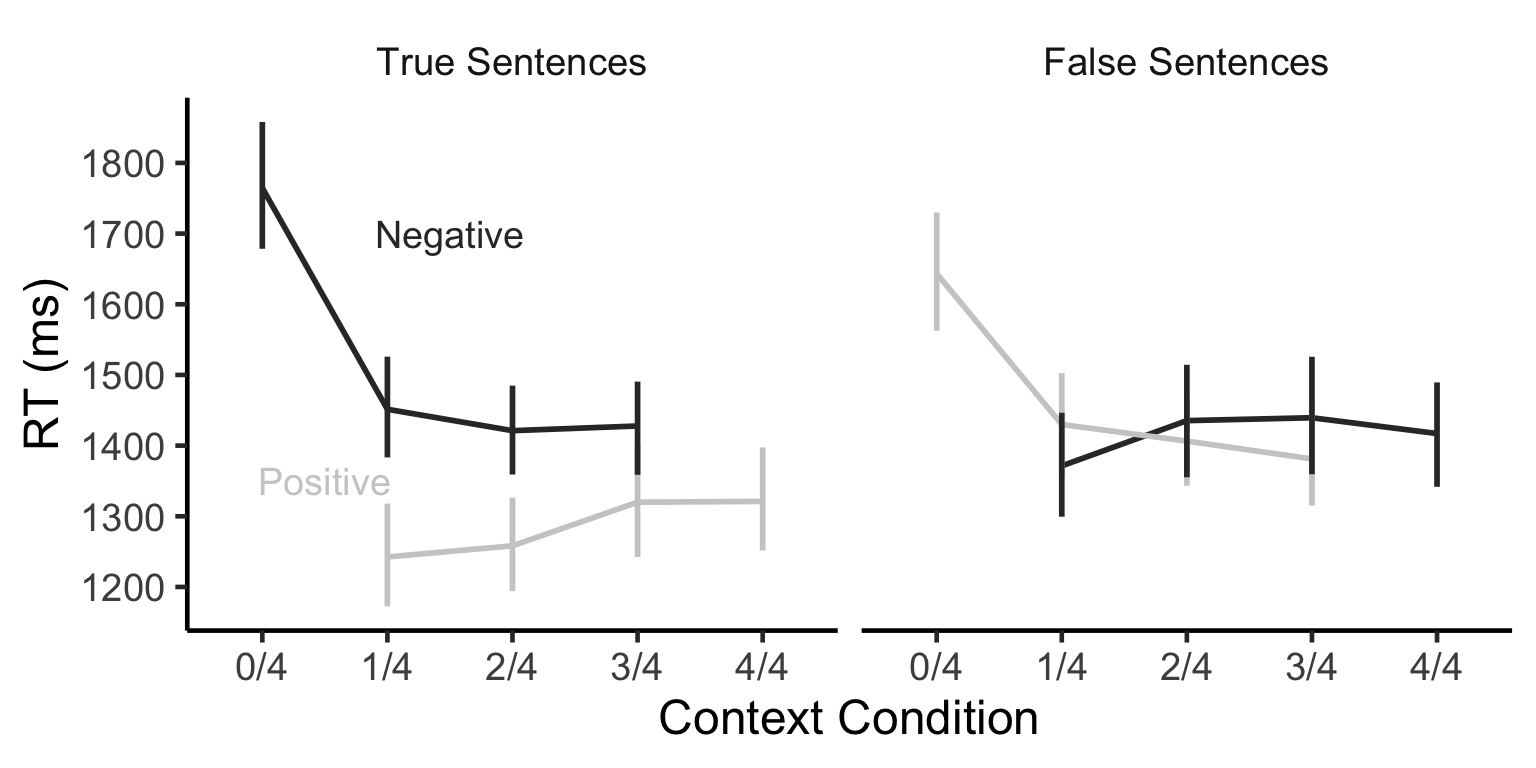
\includegraphics[width=6in]{figures/experiment2/listener_rts.png}
\caption{\label{fig:exp2_listenerrt} Reaction times for each trial type across different conditions. Responses to true sentences are shown on the left, and false sentences are shown on the right.  Negative sentences are shown in black, and positive sentences in grey.  The context is notated by a fraction representing the number of characters in the context who held target items. Error bars show 95\% confidence intervals computed by non-parametric bootstrap.}
\end{center} 
\end{figure}

Overall accuracy on this task was again very high, with participants responding correctly on 98\% of true positive trials, 93\% of true negative trials, 96\% of false positive trials, and 97\% of false negative trials. Reaction times for Experiment 2b can be seen in Figure \ref{fig:exp2_listenerrt}. As in Experiment 1b, we again see main effects of sentence type, with participants responding faster to positive sentences than negative sentences, and an interaction between truth value and polarity. We also see again that the $\frac{0}{4}$ context yields much slower reaction times than any other context, suggesting again a striking effect of relevance on both true negative and false positive sentences. 

We fit a linear mixed-effects model to examine the interaction between sentence type (positive or negative), truth value (true or false), and context as predictors of reaction time.\footnote{The model specification was as follows: \texttt{RT $\sim$ sentence~$\times$~truth~$\times$~context + (sentence~\textbar~subject) +  (sentence~\textbar~item)}.} All model coefficients are shown in Table \ref{tab:exp2_listenermodel}. In addition to main effects of sentence type ($\beta= -205$, $p< .001$) and truth value ($\beta= -384$, $p< .001$), there was an interaction such that true positive sentences elicited the fastest responses and true negative sentences elicited the slowest responses ($\beta= 663$, $p< .001$). The model showed a significant negative linear effect of context, with reaction times decreasing as the proportion of characters with target items increased ($\beta= -341$, $p< .001$). A significant three-way interaction between sentence type, truth value, and context indicates that this pattern was driven primarily by responses to true negative sentences, with context having the most pronounced effect on true negative utterances ($\beta= -901$, $p< .001$).  

To explore the separate effects of relevance (i.e., the effect of the $\frac{0}{4}$ context compared to the others) and informativeness (i.e. the linear effect of context) on responses to true utterances, we fit two separate models to reaction times in response to true positive and true negative utterances.\footnote{Model specification for true negative model: \texttt{rt $\sim$  relevance context + numeric context + (relevant context + numeric context~\textbar~subject) +  (relevant context + numeric context~\textbar~item)}; model specification for true positive model: \texttt{rt $\sim$  numeric context + (numeric context~\textbar~subject) +  (numeric context~\textbar~item)}.} We found a significant effect of relevance on reaction times for negative utterances, with the $\frac{0}{4}$ context producing significantly slower reaction times compared to the relevant contexts ($\beta= 307$, $p< .001$). We did not find a significant linear effect of context above and beyond the effect of the  $\frac{0}{4}$ context ($\beta= -41$, $p = .58$). We did, however, find a significant positive linear effect of context on the the reaction time to respond to positive sentences ($\beta= 111$, $p = .02$), indicating a significant effect of informativeness on RTs to positive sentences, but not negative sentences. 

\begin{table}
\caption{\label{tab:exp2_listenermodel} Model output from a mixed-effects model predicting listeners' reaction times in response to sentences in different contexts.}
\begin{center}
% \small\addtolength{\tabcolsep}{-5pt}
\begin{tabular}{rrrr}
  \hline
 & Coefficient & Std. err. & $t$ \\ 
  \hline
Intercept & 1598 & 41 & 39.16 \\ 
  Sentence (Negative) & -205 & 38 & -5.36  \\ 
  Truth (True) & -384 & 36 & -10.57 \\
  Context & -341 & 42 & -8.14 \\ 
  Sentence $\times$ Truth & 663 & 54 & 12.16 \\
  Sentence $\times$ Context & 377 & 59 & 6.40 \\
  Truth $\times$ Context & 454 & 59 & 7.71 \\
  Sentence $\times$ Truth $\times$ Context & -901 & 83 & -10.79 \\
   \hline
\end{tabular}
\end{center}
\end{table}


\subsubsection{Comparing Speakers and Listeners across Experiment 2}

\begin{figure}[t]
\begin{center} 
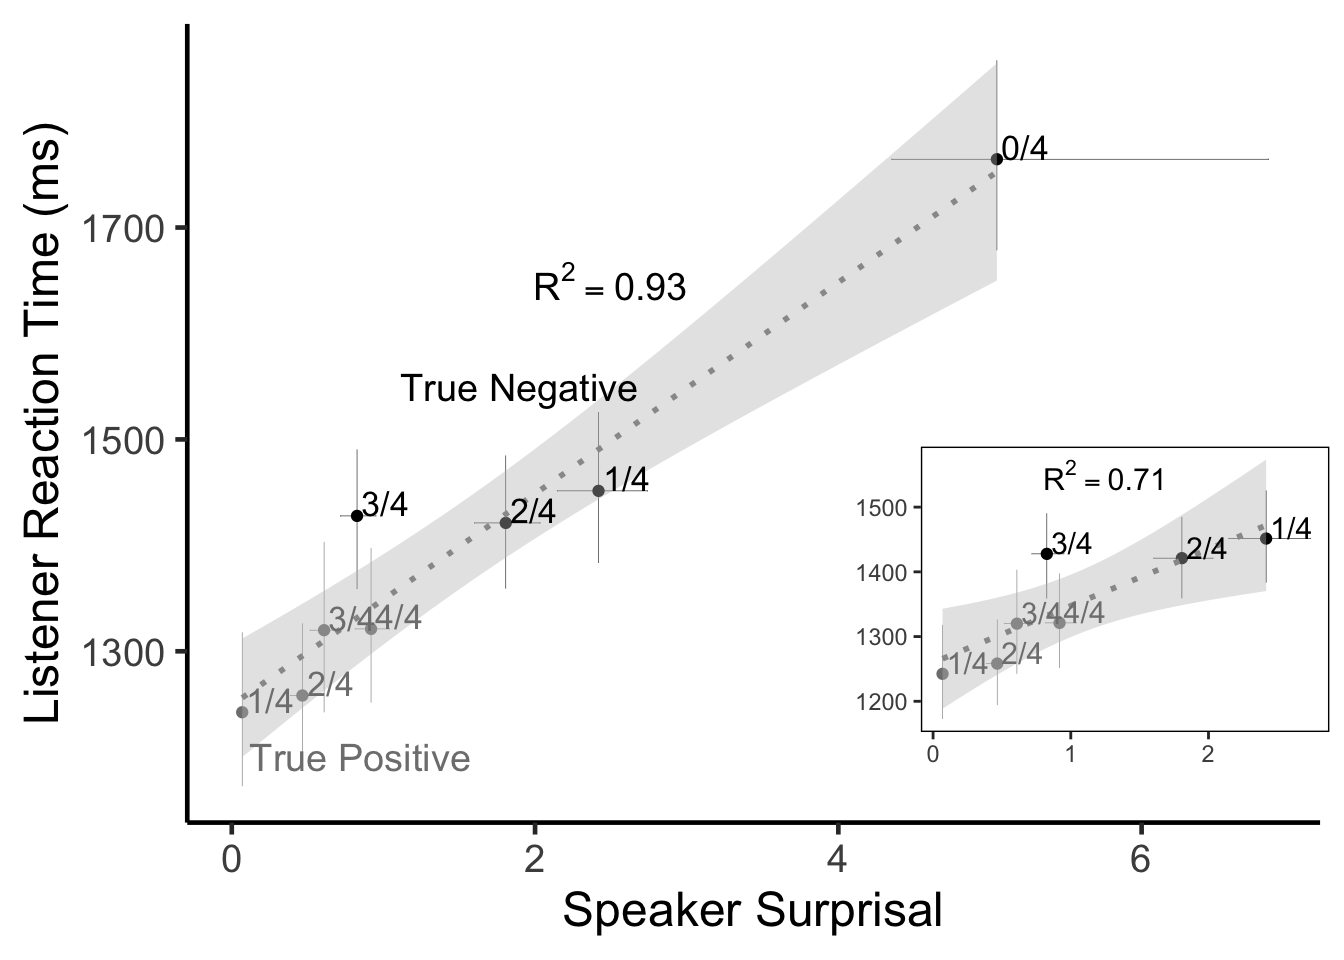
\includegraphics[width=6in]{figures/experiment2/speaker_v_listener.png}
\caption{\label{fig:exp2_scatter} Reaction times in the listener condition plotted by surprisal in the speaker condition. Each point represents a measurement for sentence type and context. Negative sentences are shown in black, and positive sentences in grey. Error bars on the horizontal and vertical axes represent 95\% confidence intervals on their respective measures. The gray band shows the linear regression and  95\% confidence region for all conditions. The inset graph zooms in on the linear regression and 95\% confidence region for data excluding the outlying 0/4 condition.}
\end{center} 
\end{figure}

As in Experiment 1, we regressed the mean reaction time in response to true positive and negative utterances in each condition against the surprisal for the same utterances in order to test our hypothesis that processing times are a function of listeners' expectations about what a speaker will say (Figure \ref{fig:exp2_scatter}).  There was a significant positive relationship between surprisal and reaction time for true negative sentences, $R^2=.93$, $p<.001$, supporting our prediction that the effects of context on reaction time reflect differences in how speakers would describe the same stimuli. This relationship between surprisal and reaction time for true negative sentences holds even with the outlying $\frac{0}{4}$ context removed from analysis ($R^2=.71$, $p = .017$).

\section{General Discussion}

What makes negation hard to process? Our work suggests that the same general pragmatic mechanisms that govern positive sentences are responsible for much of the difficulty associated with negative sentences. Negative sentences presented without context are uninformative and not relevant; thus, they are unlikely to be produced by speakers. In turn, listeners respond to unlikely utterances with increased processing times. In contexts where negation is relevant and more informative, processing costs are lower. Overall, this evidence supports a Gricean interpretation of negation processing, with pragmatic principles playing a role in the processing of both positive and negative sentences.

While previous work has shown that contextual factors facilitate the processing of negation \cite{wason1965,nieuwland2008,dale2011,orenes2014}, our findings here go further. First, by using actual language productions as the predictor of processing difficulty, our work implicates specifically pragmatic factors. Because the field of pragmatics is concerned with language \textit{use}, demonstrating a relationship between actual speaker productions and listener processing time is critical to the argument that pragmatic factors are responsible for the processing cost of negation. Second, rather than treating pragmatics as a black box, we show that two different components---informativeness and relevance---each contribute to the relative (un-)likelihood of hearing a negation. Speakers in both experiments were unlikely to mention the absence of a feature unless it was a relevant response to a likely QUD, and were more likely to mention the presence or absence of features when mentioning those features would help uniquely identify the referent. The fact that informativeness played a role in the production of both positive and negative utterances supports our argument that these pragmatic pressures are general, rather than specific to negation. 

Speakers in both experiments were most likely to produce true negatives in the $\frac{1}{4}$, $\frac{2}{4}$, and $\frac{3}{4}$ contexts. As suggested in \citeA{xiang2020}, these are contexts that give rise to a polar QUD. The structure of the experiment may have also played a role in QUD inference; e.g., our prompt for speakers asked them to fill in the sentence ``[NAME] has $\rule{3cm}{0.15mm}$.'' which may have biased speakers towards a polar QUD (e.g. \textit{Does [NAME] have [ITEM]?}). The within-subjects structure may also have contributed to this, as participants may have inferred the polar QUD due to the presence/absence of items varying across different trials.

% Informativeness predicts that speakers should produce utterances that are maximally helpful in allowing the listener to identify the referent of a sentence.
% ; our data suggests that speakers are increasingly likely to describe a character by negating the target feature as the number of context characters \textit{with} the target feature increases.  
% Furthermore, the low probability (and corresponding slow reaction time) of participants producing true negative sentences in the $\frac{0}{4}$ context suggests that speakers are unlikely to produce negation unless there is a relevant feature to negate.

Listeners' reaction times were highly correlated with the surprisal of a speaker producing the same utterances in context in both Experiment 1b and Experiment 2b. For true negative sentences, however, this effect was driven primarily by the effect of relevance (i.e., the difference between the $\frac{0}{4}$ and all other contexts). Why didn't informativeness play a role in listeners' response times? One possibility is that only relevance plays a role in forming listeners' expectations about what a speaker will say. Another possibility is that the effect of informativeness is small compared to the effect of relevance, and that the reaction time measure is too noisy to identify this effect. Although our results cannot disentangle these two possibilities, the fact that we did find a significant effect of informativeness on listeners' responses to true positive sentences suggests that informativeness does play some role in listeners' expectations. 

One possible explanation for the difference in reaction time between the $\frac{0}{4}$ context and the other contexts is that in the contexts where apples are present, the visual presence of apples primes the semantic processing of sentences with the word ``apples'' (see e.g.,\citeNP{sperber1979}). In our experiments, we cannot disentangle the possible lower-level effect of this type of lexical activation from the facilitation that comes from listener expectations about what a speaker might say. What it means for a word or sentence to be facilitated by ``predictability'' likely occurs at multiple levels of representation. That is, the lower-level semantic priming that might occur upon seeing a picture of an apple might facilitate the higher-level expectations that a listener makes about a speaker utterance (see \citeNP{kuperberg2016} for a discussion of prediction at multiple levels of representation). 

Much like other psycholinguistic experiments, our tasks take place in a restricted world where the set of possible referents (and by extension, the set of possible utterances that a speaker is likely to produce) is limited. In real world contexts, a speaker could produce many different utterances to describe many different referents at any given moment. Our goal in these experiments is to explore whether Neo-Gricean pragmatic principles can at minimum explain how people communicate in these restricted worlds. Our theory would predict that when people produce negative utterances in the ``real world'' they are \textit{usually} producing them in contexts where those utterances are highly informative and relevant; thus, we would predict that people have less difficulty processing negative sentences in natural conversation than they do in constrained psycholinguistic experiments.

%We use surprisal, an information-theoretic measure of processing difficulty, as the linking hypothesis between speaker probabilities and reaction times \cite{levy2008}. Although this link has substantial support in the realm of syntactic processing \cite{demberg2008,boston2008}, to our knowledge, our findings are the first example of using surprisal over sentence-level pragmatic expectations, rather than word-level syntactic expectations. This success suggests that, in concert with the appropriate predictive models, surprisal theory could be productively applied to the prediction of processing difficulty beyond the level of syntax. 

Our analysis is intended as a computational level analysis \cite{marr1982}. We are not committed to a specific account of how negative sentences or pragmatic inferences are represented. Our results don't tell us whether listeners actually simulate a speaker or a specific QUD when they form expectations about what a speaker will say, or doing something that approximates such a simulation. Our goal is to show at least that the weaker of these two possibilities is true; that is, listeners are forming expectations about what a speaker will say, even though we don't know precisely what form these representations take. Several mechanistic theories of pragmatics have been proposed, such as an in-the-moment alignment of linguistic representations between speakers and listeners \cite{pickering2004}, or cached expectations about how speakers use language leading to preferred interpretations by listeners \cite{levinson2000}. Either of these possibilities, or any number of others, could be consistent with our data. 

In the domain of negation, a number of theories have been proposed to explain how negation is represented and processed at the mechanistic level. Two-step theories of negation processing have argued that negation is processed by first representing the negated state of affairs, and then rejecting this in favor of the actual state of affairs; these representations have been argued by some to be propositional in nature \cite{hclark1972} or simulations of the true and negated state of affairs \cite{kaup2003, kaup2006, kaup2007}. These theories can explain why, in many tests of negation processing -- including ours -- there is an interaction between the polarity and truth value of a sentence. Other theories argue that under the right experimental and pragmatic conditions, the true state of affairs is represented and accessible to comprehenders immediately, suggesting that it is possible for negation to be processed fluently in a single step, especially in supportive contexts (as is also reflected in the contexts effects seen in our data, though we note that even in our most supportive contexts, negation was processed slower) \cite{tian2010, tian2016, papeo2016, wang2021}. Although this body of literature is highly complementary to the data we have presented here, our studies here are not designed to test between competing theories about the mechanism by which negation is represented. 

Although we focus here on negation, our findings have implications for sentence processing more generally.  Debates about the effects of pragmatics on linguistic processing exist in other domains, such as the processing of scalar implicatures \cite<the pragmatic inference that e.g., ``some'' implicates ``some but not all'';>{huang2009, huang2011, grodner2010}.  \citeA{tomlinson2013} provide an informative comparison between scalar implicature and negation, presenting mouse-tracking trajectories for each. Their negation data show the same pattern of processing difficulties we observe, and critically, their data on the processing of underinformative ``some'' utterances look almost identical. We hypothesize that, in both cases, participants' processing difficulty is a function of the violation of their pragmatic expectations about what speakers will say.

Our findings here suggest that the processing difficulties of negative sentences arise at least in part from the relative pragmatic felicity of negation in context. Neo-Gricean principles of informativeness and relevance impact the probability of producing negative sentences in different contexts, and listeners expect speakers to abide by these principles. This finding leads us to the following conclusion: When logical words are used in a communicative context, we have no difficulty understanding them.

\subsection{Author Contributions}
Both authors developed the study concept and contributed to the study design.  Data collection was conducted by AEN.  AEN performed the data analysis and interpretation under the supervision of MCF.  Both authors contributed to the development of the manuscript and approved the final version of the manuscript for submission.

\subsection{Funding Information}
This work supported by the NSF GRFP to AEN and ONR N00014-13-1-0287.

\subsection{Competing Interests}
The authors declare no competing interests. 

\subsection{Data Accessibility Statement} 
All the stimuli, experiment code, raw data, and analysis scripts described here can be found in the supplemental materials on this paper's project page at \url{https://github.com/anordmey/negatron}. 


%  show the same mouse-tracking patterns in response to underinformative scalar implicatures as well as underinformative negative utterances.  

% We believe that formal models of pragmatics can provide insight into these debates and, more generally, into the role that pragmatic context plays in linguistic processing. 

% One contribution of our work here is that we use language production behavior to provide a strong operational definition of pragmatics.  Building on recent 

 % modeling work quantifies pragmatic reasoning based on the assumption that speakers are informative---they will produce utterances that pick out smaller subsets of the context, leaving as little ambiguity as possible for the listener \cite{frank2012,goodman2013}.  By this definition, negative sentences become more informative as the number of characters in the context increases.  This prediction is reflected in our results: Speakers were more likely to use negation in contexts where more people possessed the negated item.  

% We also found that both speakers' and listeners' behavior was strongly influenced by the presence of any target items in the context.  Speakers were much less likely to produce a negative utterance when none of the characters in the context possessed target objects; similarly, listeners took much longer to respond to these sentences than any of the other contexts.  We saw the same pattern in listeners' responses to false negative sentences.  These findings are consistent with relevance theory \cite{sperber1986}, as well as the idea that a speakers' utterances are influenced by the ``Question Under Discussion'' \cite{roberts1996}.  In addition to being uninformative, a sentence such as ``Bob has/has no apples'' in a context where none of the characters have apples is very strange, because ``apples'' is not a relevant feature of the context.  We interpret this finding as evidence for the role of relevance in producing and processing speech; in addition to being uninformative, these sentences might have incurred additional processing costs due to the mention of an unexpected topic.    

%Our analyses focused on true sentences, because of our interest in exploring participants' expectations about how an informative speaker should behave.  Due to the nature of our task, participants in the listener condition likely expected some of the sentences to be false, but it is not clear what constitutes an ``informative'' false sentence.  Our listener data replicate an interaction between sentence type and truth value that is seen frequently in literature on sentence verification tasks \cite{hclark1972}, with false positive sentences showing a similar pattern as true negative sentences.  




% These were contexts in which negation was informative (i.e., identified a narrower subset of the context) and relevant (i.e., the negated item was present in the context).  This pattern was also consistent with our Gricean hypothesis that the processing cost of negation is due to general pragmatic principles about how listeners expect speakers to behave.  

% In conversation, in contrast, negative sentences are often produced when some strong expectation has been violated, making the negation both informative and relevant. Congruent with that impression, 

% Our participants were faster to respond to negative sentences in contexts where speakers were more likely to use negation to describe the same stimuli. 

%We suggested a Gricean account of these data: The processing cost of negation is related to the degree to which it violates expectations about communication in context. In our studies, by changing the proportion of people in the context who held a target item, we systematically manipulated participants' contextual expectations.  We found a parametric relationship between the strength of the context and reaction times, and this relationship was well fit by participants' descriptions of the stimuli in different contexts.


 
 % and slower processing times.  


\bibliographystyle{apacite}

\setlength{\bibleftmargin}{.125in}
\setlength{\bibindent}{-\bibleftmargin}

\bibliography{negation}



\end{document}


%Maybe move some of this to the GD
%What is the mechanism by which context influences the processing of negation?  We propose that negative sentences are more informative in contexts that set up a strong expectation that is violated. If the processing cost of negation is pragmatic, then more informative negative sentences should elicit smaller reaction times. How should we quantify informativeness in context? Recent modeling work quantifies pragmatic reasoning in simple experimental contexts \cite{frank2012,goodman2013}. The assumption underlying this work is that speakers are informative---they will produce utterances that will pick out smaller subsets of the context, leaving as little ambiguity as possible for the listener.  We use this definition of informativeness to provide a quantitative interpretation of our hypothesis.

%MOVE THIS:
%To link pragmatic expectations to reaction time, we assume that reaction time is proportional to \textit{surprisal}. Surprisal is an information-theoretic measure of the amount of information carried by an event (in this case, an utterance in some context) based on its probability. Surprisal has been used effectively to predict reaction times from probabilistic models \cite{levy2008}; in this work, we directly measure the probability of an utterance occurring by eliciting descriptions of our stimuli from our participants.